\documentclass{beamer}
\usepackage[utf8]{inputenc}
\usepackage{graphicx, epsfig}
\usepackage{amsmath,mathrsfs,amsfonts,amssymb}
%\usepackage{subfig}
\usepackage{floatflt}
\usepackage{epic,ecltree}
\usepackage{mathtext}
\usepackage{fancybox}
\usepackage{fancyhdr}
\usepackage{multirow}
\usepackage{enumerate}
\usepackage{epstopdf}
\usepackage{multicol}
\usepackage{algorithm}
\usepackage[noend]{algorithmic}
\usepackage{tikz}
\usepackage{blindtext}
\usetheme{default}%{Singapore}%{Warsaw}%{Warsaw}%{Darmstadt}
\usecolortheme{default}
\setbeamerfont{title}{size=\Huge}
\setbeamertemplate{footline}[page number]{}


\makeatletter
\newcommand\HUGE{\@setfontsize\Huge{35}{40}}
\makeatother    

\setbeamerfont{title}{size=\HUGE}
\beamertemplatenavigationsymbolsempty

% latin bold lower
\newcommand{\ba}{\mathbf{a}} 
\newcommand{\bc}{\mathbf{c}} 
\newcommand{\be}{\mathbf{e}} 
\newcommand{\bh}{\mathbf{h}} 
\newcommand{\bp}{\mathbf{p}} 
\newcommand{\bt}{\mathbf{t}} 
\newcommand{\bs}{\mathbf{s}} 
\newcommand{\bu}{\mathbf{u}} 
\newcommand{\bv}{\mathbf{v}} 
\newcommand{\bw}{\mathbf{w}} 
\newcommand{\bx}{\mathbf{x}} 
\newcommand{\by}{\mathbf{y}} 
\newcommand{\bz}{\mathbf{z}} 

% latin bold upper
\newcommand{\bA}{\mathbf{A}} 
\newcommand{\bB}{\mathbf{B}} 
\newcommand{\bC}{\mathbf{C}} 
\newcommand{\bI}{\mathbf{I}} 
\newcommand{\bL}{\mathbf{L}} 
\newcommand{\bM}{\mathbf{M}} 
\newcommand{\bQ}{\mathbf{Q}} 
\newcommand{\bT}{\mathbf{T}} 
\newcommand{\bU}{\mathbf{U}} 
\newcommand{\bV}{\mathbf{V}} 
\newcommand{\bW}{\mathbf{W}} 
\newcommand{\bX}{\mathbf{X}} 
\newcommand{\bY}{\mathbf{Y}} 
\newcommand{\bZ}{\mathbf{Z}} 

% latin cal upper
\newcommand{\cG}{\mathcal{G}} 
\newcommand{\cL}{\mathcal{L}} 
\newcommand{\cN}{\mathcal{N}} 
\newcommand{\cS}{\mathcal{S}} 
\newcommand{\cT}{\mathcal{T}} 
\newcommand{\cW}{\mathcal{W}} 
\newcommand{\cX}{\mathcal{X}} 
\newcommand{\cZ}{\mathcal{Z}} 

% latin bb upper
\newcommand{\bbE}{\mathbb{E}} 
\newcommand{\bbI}{\mathbb{I}} 
\newcommand{\bbP}{\mathbb{P}} 
\newcommand{\bbR}{\mathbb{R}} 

% greek bold lower
\newcommand{\bepsilon}{\boldsymbol{\epsilon}} 
\newcommand{\btheta}{\boldsymbol{\theta}} 
\newcommand{\blambda}{\boldsymbol{\lambda}} 
\newcommand{\bpi}{\boldsymbol{\pi}} 
\newcommand{\bmu}{\boldsymbol{\mu}} 
\newcommand{\bsigma}{\boldsymbol{\sigma}} 
\newcommand{\bphi}{\boldsymbol{\phi}} 

% greek bold upper
\newcommand{\bSigma}{\boldsymbol{\Sigma}} 

\DeclareMathOperator*{\argmin}{arg\,min}
\DeclareMathOperator*{\argmax}{arg\,max}

\newcommand{\createdgmtitle}[1]{\title[\hbox to 56mm{Deep Generative Models  \hfill\insertframenumber\,/\,\inserttotalframenumber}]
	{\vspace{1.5cm} \\ Deep Generative Models \\ {\Huge Lecture #1}}
	\author{Roman Isachenko}
	\institute{
	Moscow Institute of Physics and Technology
	} 
	\date{Autumn, 2021}
}

\newcommand\myfootnote[1]{%
  \tikz[remember picture,overlay]
  \draw (current page.south west) +(1in + \oddsidemargin,0.5em)
  node[anchor=south west,inner sep=0pt]{\parbox{\textwidth}{%
      \rlap{\rule{10em}{0.4pt}}\raggedright\scriptsize \textit{#1}}};}

\newcommand\myfootnotewithlink[2]{%
  \tikz[remember picture,overlay]
  \draw (current page.south west) +(1in + \oddsidemargin,0.5em)
  node[anchor=south west,inner sep=0pt]{\parbox{\textwidth}{%
      \rlap{\rule{10em}{0.4pt}}\raggedright\scriptsize\href{#1}{\textit{#2}}}};}
\createdgmtitle{1}
\usepackage{tikz}

\usetikzlibrary{arrows,shapes,positioning,shadows,trees}



%--------------------------------------------------------------------------------
\begin{document}
%--------------------------------------------------------------------------------
\begin{frame}[noframenumbering,plain]
%\thispagestyle{empty}
\titlepage
\end{frame}
%=======
\begin{frame}{Generative models zoo}
	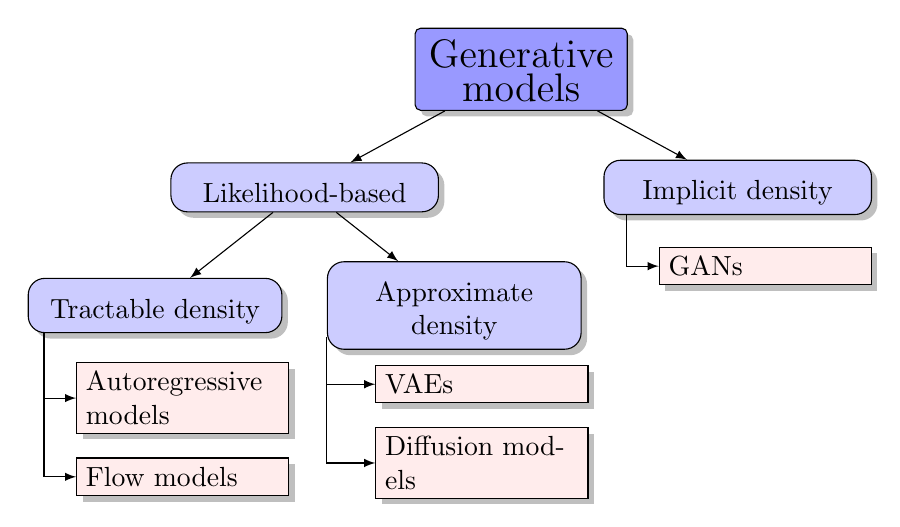
\begin{tikzpicture}[
	 	basic/.style  = {draw, text width=2cm, drop shadow, rectangle},
	 	root/.style   = {basic, rounded corners=2pt, thin, text height=1.1em, text width=7em, align=center, fill=blue!40},
	 	level 1/.style={sibling distance=55mm},
	 	level 2/.style = {basic, rounded corners=6pt, thin, align=center, fill=blue!20, text height=1.1em, text width=9em, sibling distance=38mm},
	 	level 3/.style = {basic, rounded corners=6pt, thin,align=center, fill=blue!20, text width=8.5em},
	 	level 4/.style = {basic, thin, align=left, fill=pink!30, text width=7em},
		edge from parent/.style={->,draw},
		>=latex]
		
		% root of the the initial tree, level 1
		\node[root] {\Large Generative models}
		% The first level, as children of the initial tree
		child {node[level 2] (c1) {Likelihood-based}
			child {node[level 3] (c11) {Tractable density}}
			child {node[level 3] (c12) {Approximate density}}
		}
		child {node[level 2] (c2) {Implicit density}};
		
		% The second level, relatively positioned nodes
		\begin{scope}[every node/.style={level 4}]
		\node [below of = c11, yshift=-5pt, xshift=10pt] (c111) {Autoregressive models};
		\node [below of = c111] (c112) {Flow models};
		
		\node [below of = c12, xshift=10pt] (c121) {VAEs};
		\node [below of = c121] (c122) {Diffusion models};
		
		\node [below of = c2, xshift=10pt] (c21) {GANs};
		\end{scope}
		
		% lines from each level 1 node to every one of its "children"
		\foreach \value in {1,2}
		\draw[->] (c11.194) |- (c11\value.west);
		
		\foreach \value in {1,2}
		\draw[->] (c12.194) |- (c12\value.west);
		
		\draw[->] (c2.194) |- (c21.west);
		
	\end{tikzpicture}
\end{frame}
%=======
\begin{frame}{Applications}
	\begin{figure}
		\centering
		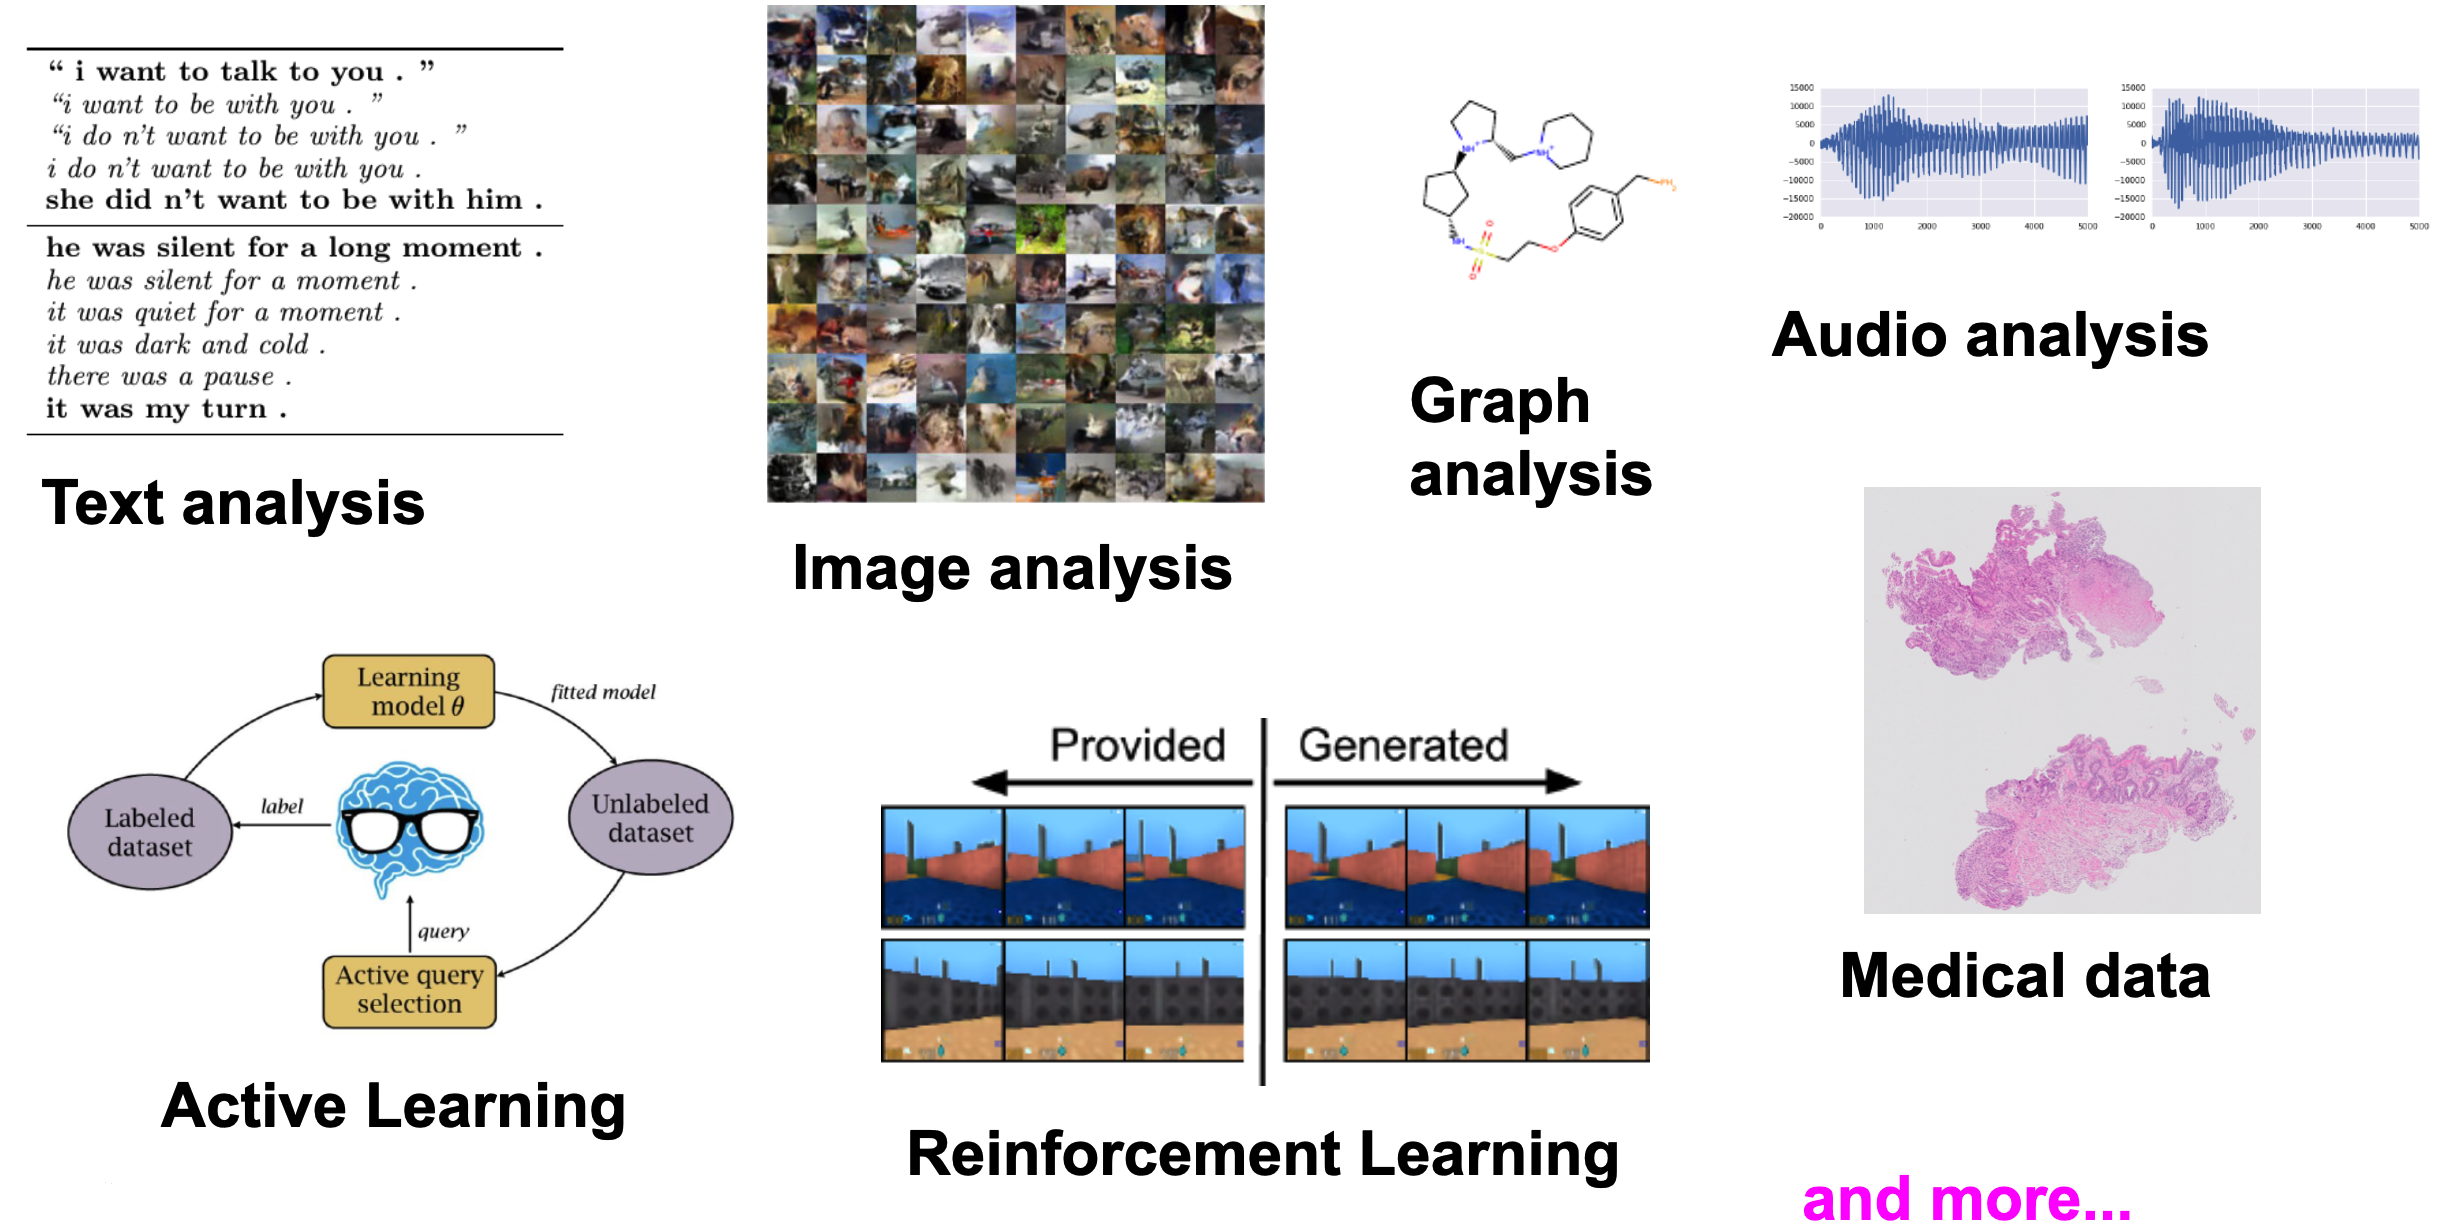
\includegraphics[width=\linewidth]{figs/applications}
	\end{figure}
	\myfootnotewithlink{https://jmtomczak.github.io/blog/1/1\_introduction.html}{image credit: https://jmtomczak.github.io/blog/1/1\_introduction.html}
\end{frame}
%=======
\begin{frame}{Applications: Image generation (VAE)}
    \begin{figure}
        \centering
        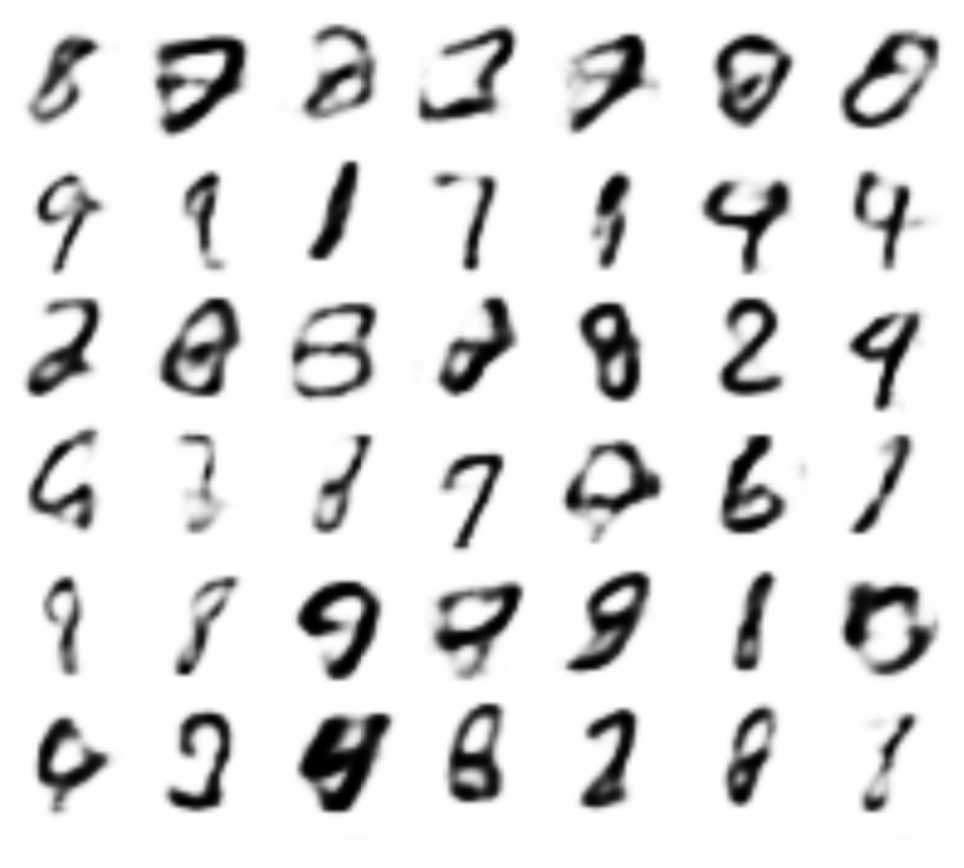
\includegraphics[width=0.8\linewidth]{figs/vae.png}
    \end{figure}
\myfootnotewithlink{https://arxiv.org/abs/1312.6114}{Kingma D. P., Welling M. Auto-encoding variational bayes, 2013}
\end{frame}
%=======
\begin{frame}{Applications: Image generation (DCGAN)}
    \begin{figure}
        \centering
        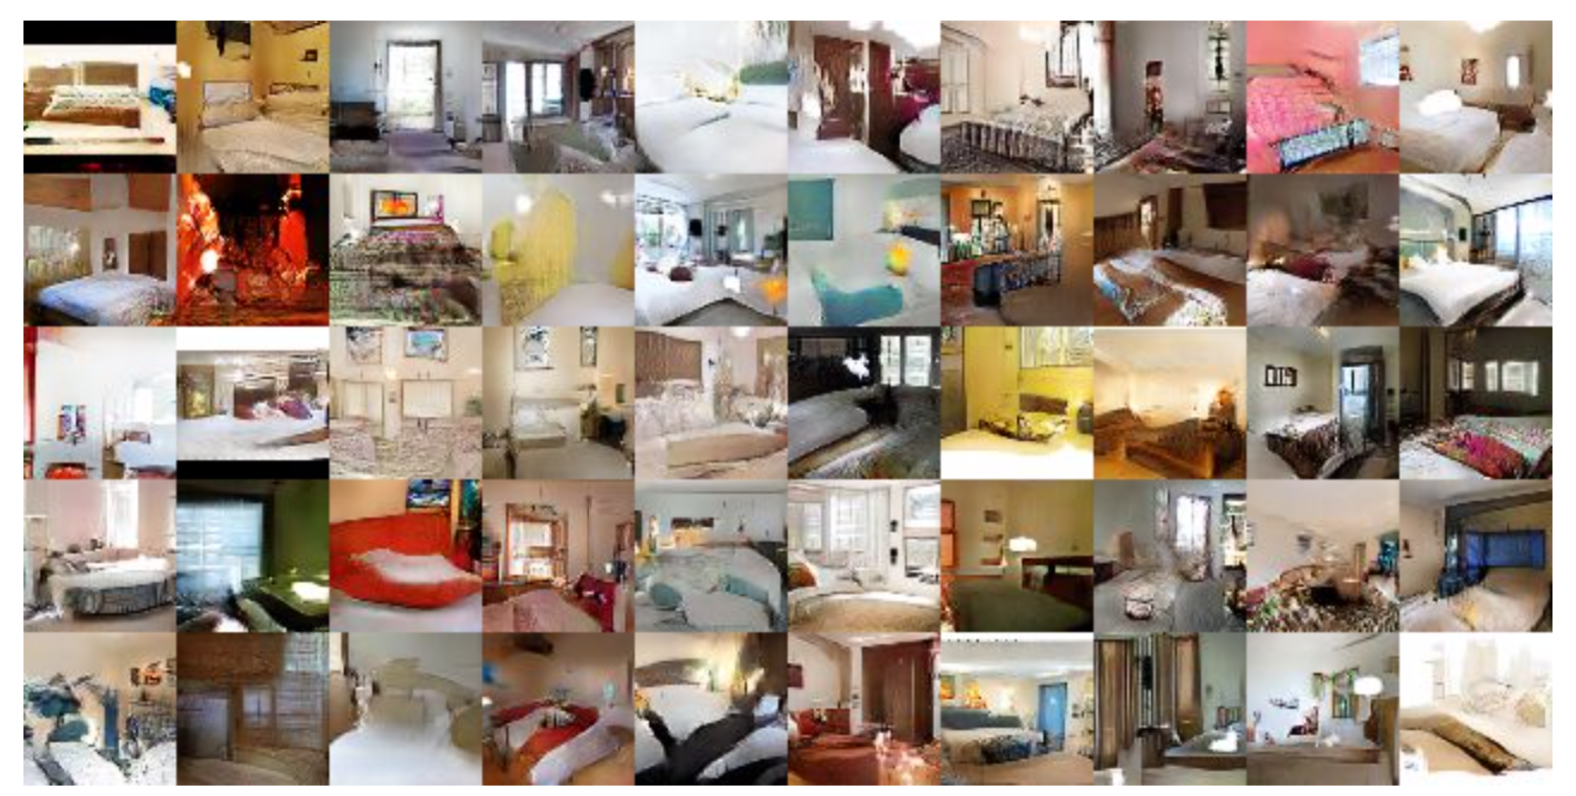
\includegraphics[width=1.0\linewidth]{figs/dcgan.png}
    \end{figure}
\myfootnotewithlink{https://arxiv.org/abs/1511.06434}{Radford A., Metz L., Chintala S. Unsupervised representation learning with deep convolutional generative adversarial networks, 2015}
\end{frame}
%=======
\begin{frame}{Applications: Face generation (StyleGAN)}
	\begin{figure}
		\centering
		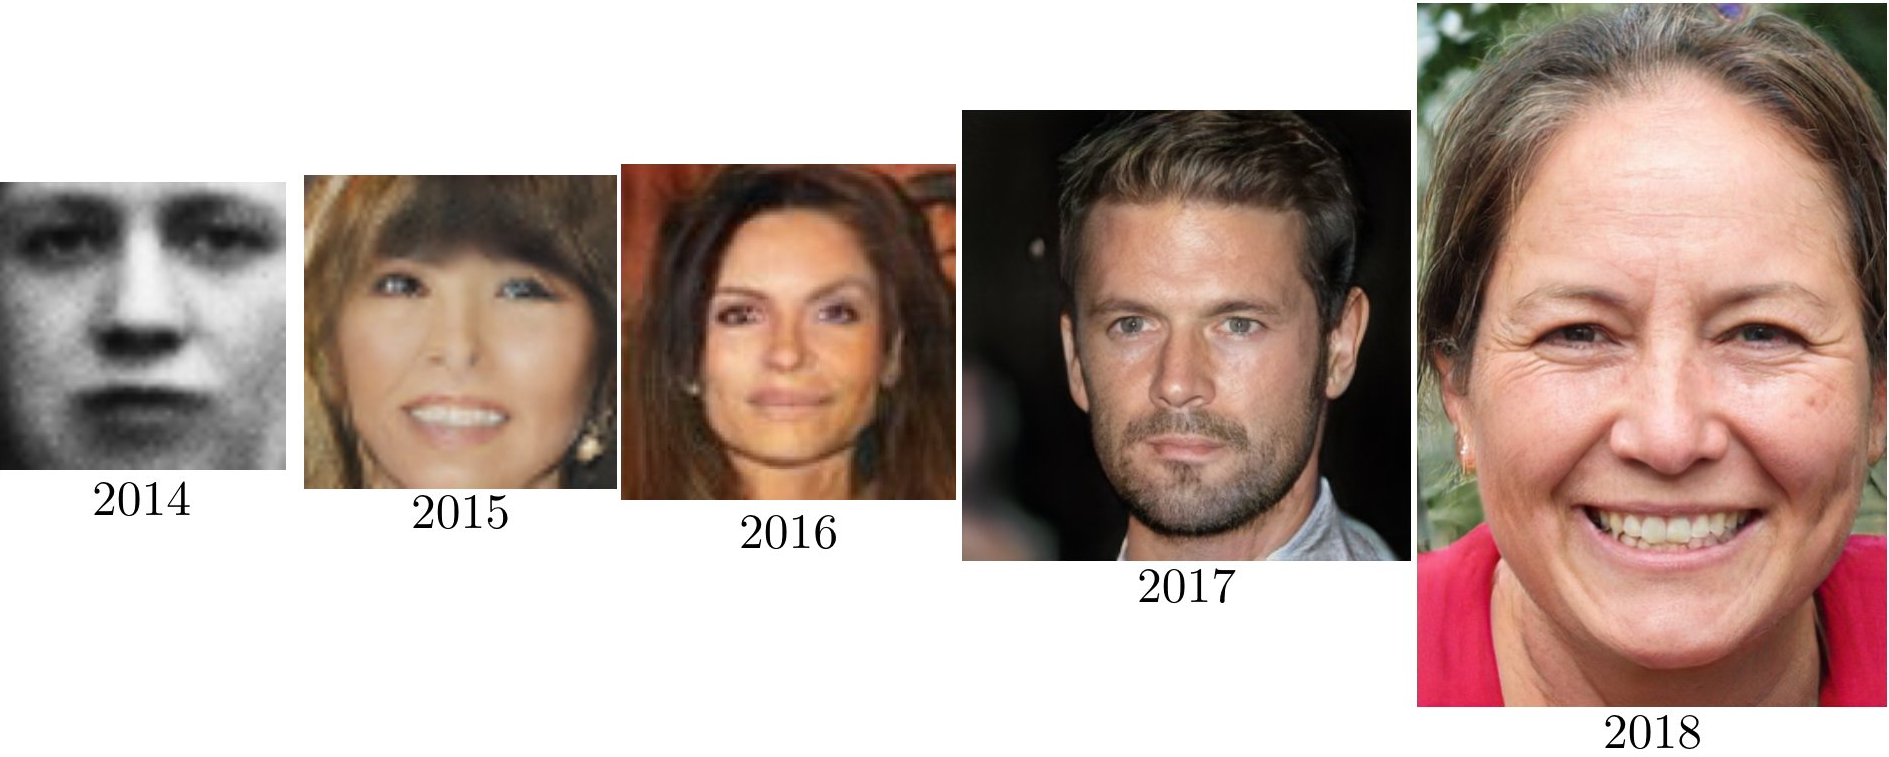
\includegraphics[width=0.85\linewidth]{figs/gan_evolution}
	\end{figure}
	\vspace{-0.2cm}
	\begin{figure}
		\centering
		\includegraphics[width=0.75\linewidth]{figs/stylegan}
	\end{figure}
	\myfootnotewithlink{https://arxiv.org/abs/1812.04948}{Karras T., Laine S., Aila T. A style-based generator architecture for generative adversarial networks, 2018}
\end{frame}
%=======
\begin{frame}{Applications: Face generation (VQ-VAE-2)}
    \begin{figure}
        \centering
        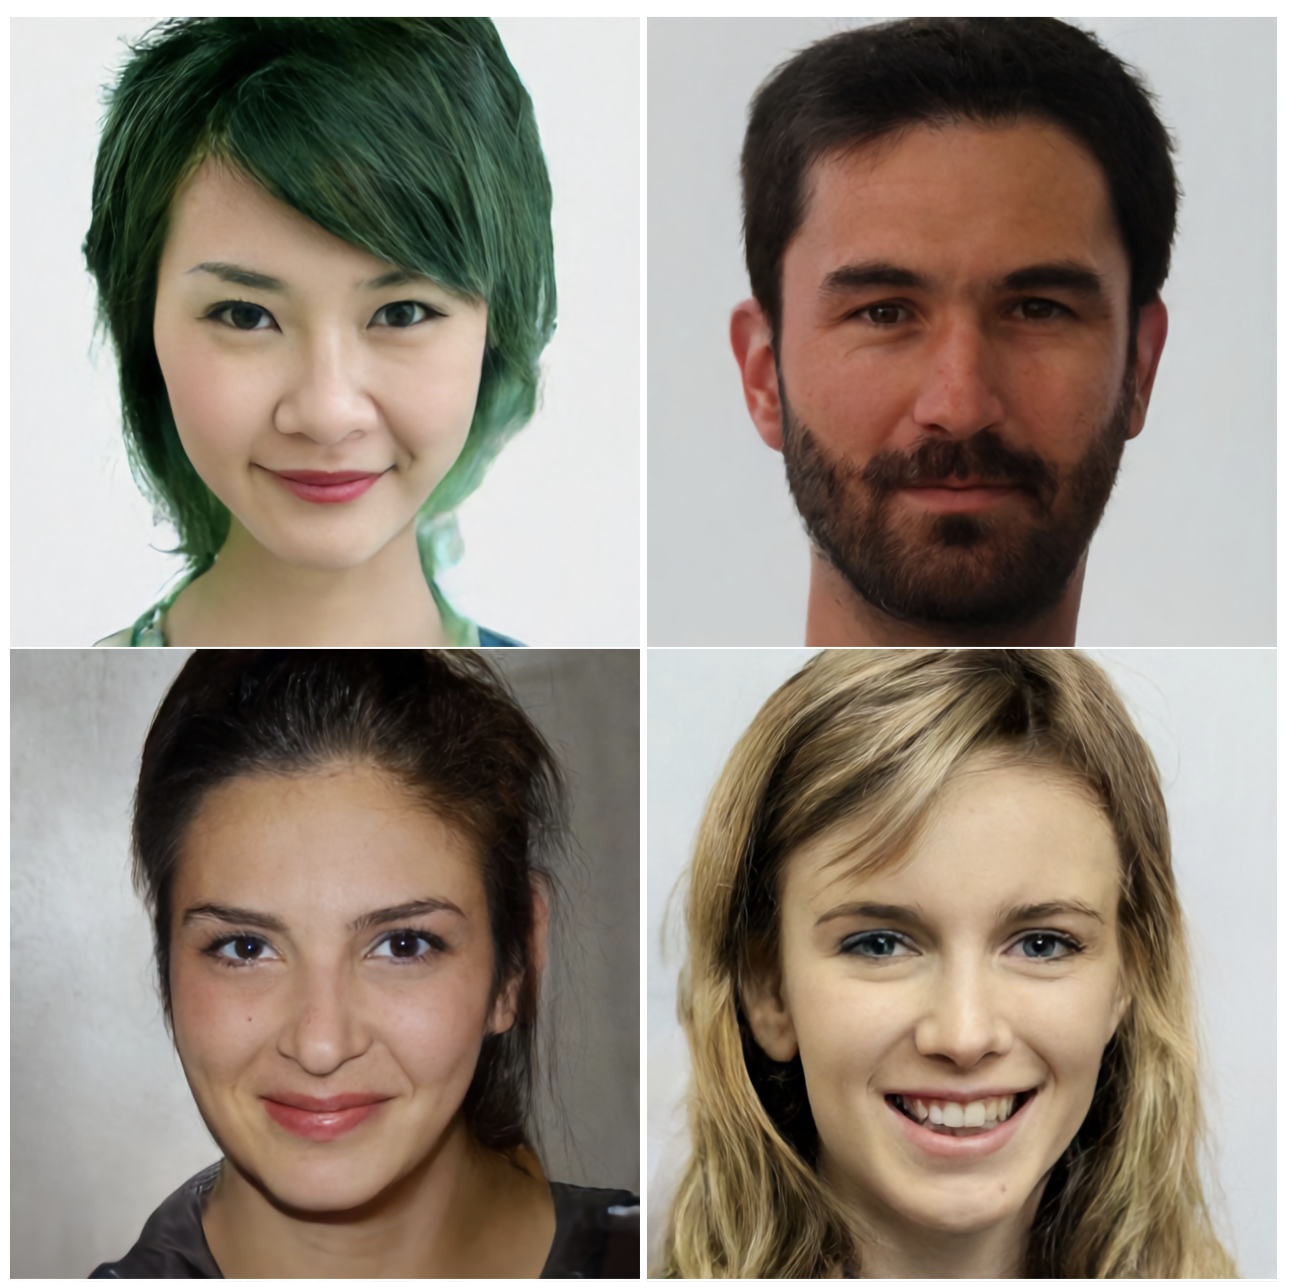
\includegraphics[width=0.7\linewidth]{figs/vq_vae.png}
    \end{figure}
\myfootnotewithlink{https://arxiv.org/abs/1906.00446}{Razavi A., Oord A., Vinyals O. Generating Diverse High-Fidelity Images with VQ-VAE-2, 2019}
\end{frame}
%=======
\begin{frame}{Applications: Language modelling}
	\begin{figure}
		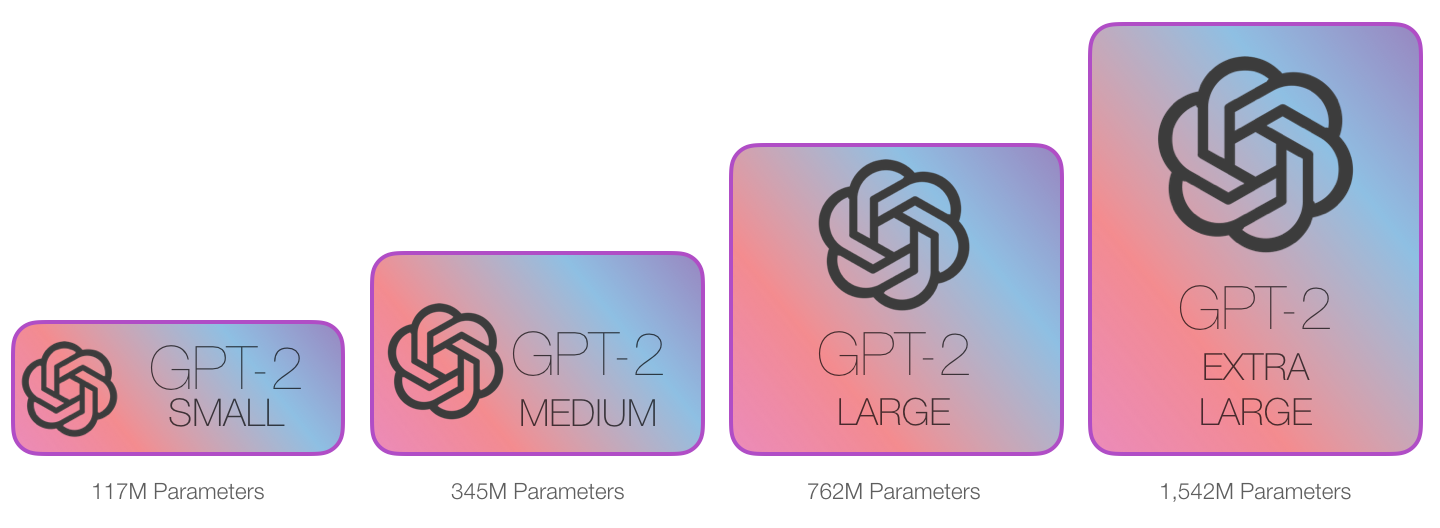
\includegraphics[width=0.65\linewidth]{figs/gpt2-sizes}
	\end{figure}
	\vspace{-0.2cm}
	\begin{figure}
		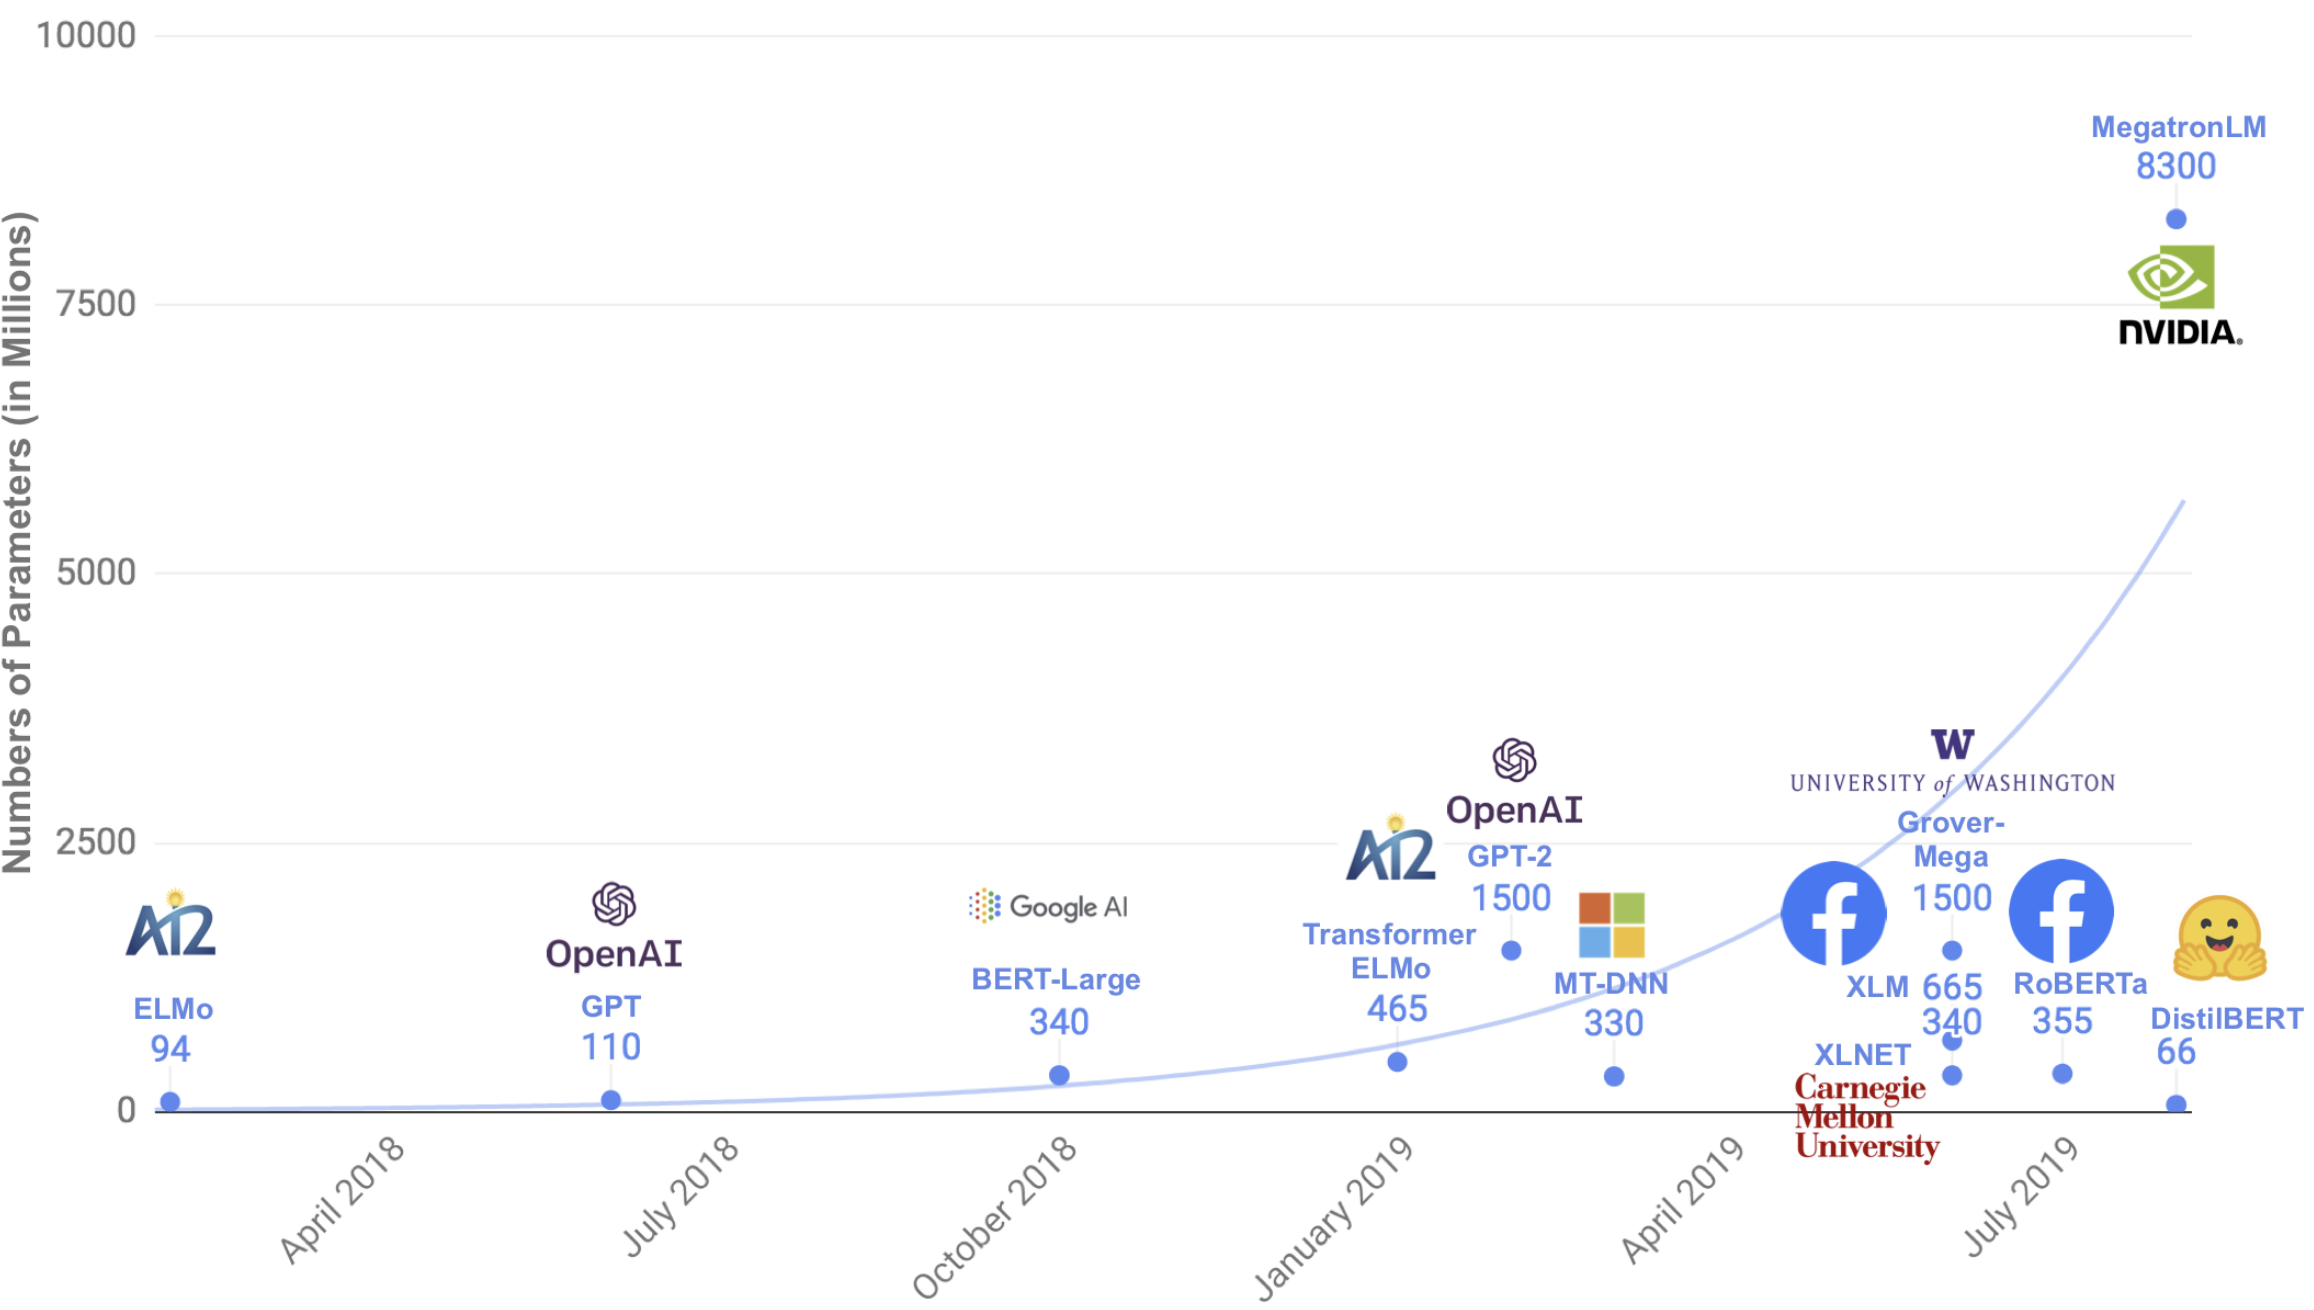
\includegraphics[width=0.7\linewidth]{figs/nlp_models}
	\end{figure}
\myfootnote{\href{http://jalammar.github.io/illustrated-gpt2}{image credit: http://jalammar.github.io/illustrated-gpt2} \\
\href{https://arxiv.org/abs/1910.01108}{Sanh V. et al. DistilBERT, a distilled version of BERT: smaller, faster, cheaper and lighter, 2019.}}
\end{frame}
%=======
\begin{frame}{Applications: Image generation, new era}
	\begin{figure}
		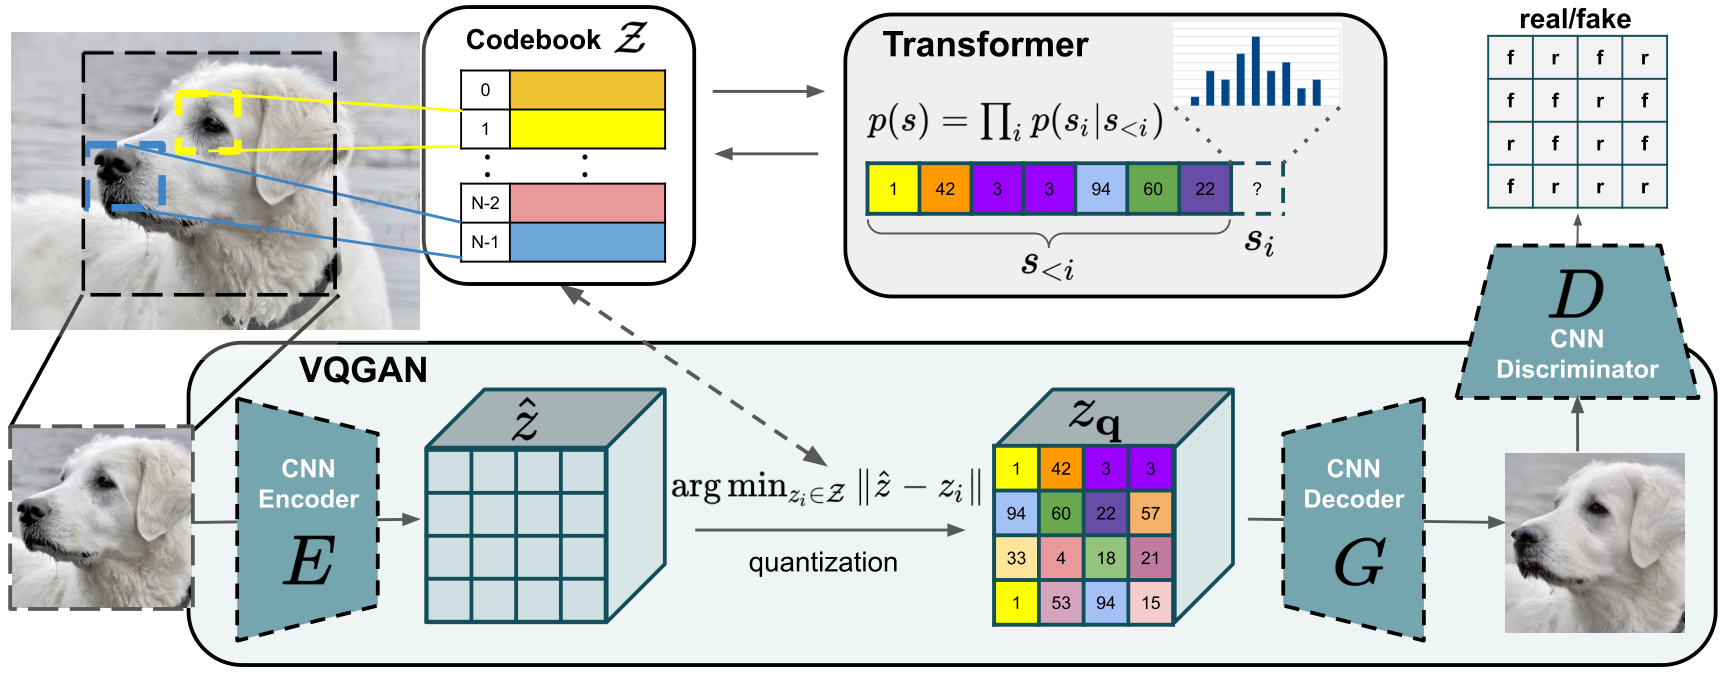
\includegraphics[width=0.8\linewidth]{figs/taming_transformers_1}
	\end{figure}
	\vspace{-0.5cm}
	\begin{figure}
		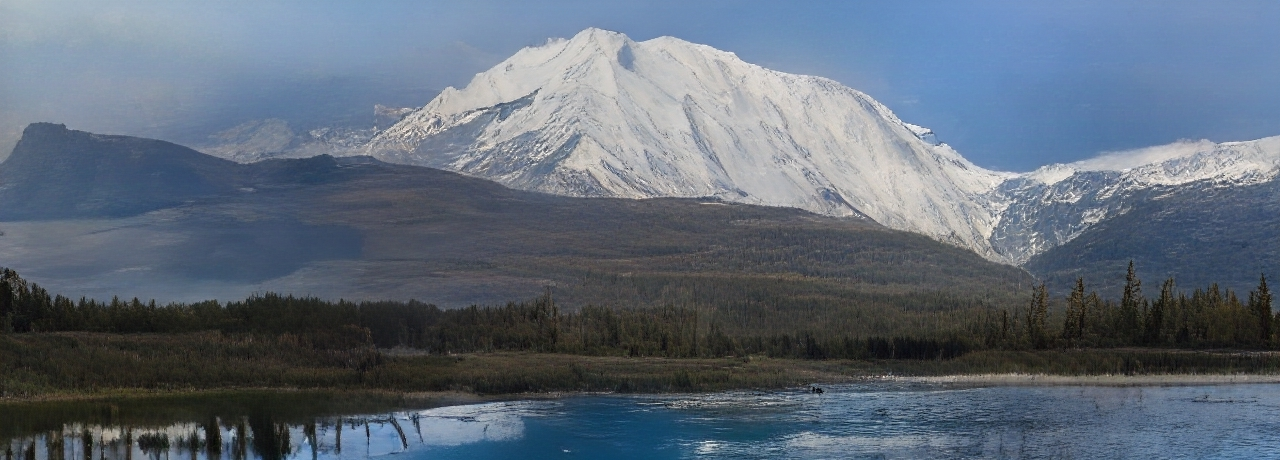
\includegraphics[width=\linewidth]{figs/taming_transformers_2}
	\end{figure}
\myfootnotewithlink{https://arxiv.org/abs/2012.09841}{Esser P., Rombach R., Ommer B. Taming Transformers for High-Resolution Image Synthesis, 2020}
\end{frame}
%=======
\begin{frame}{Applications: Cross-modal image-text models}
	\begin{figure}
		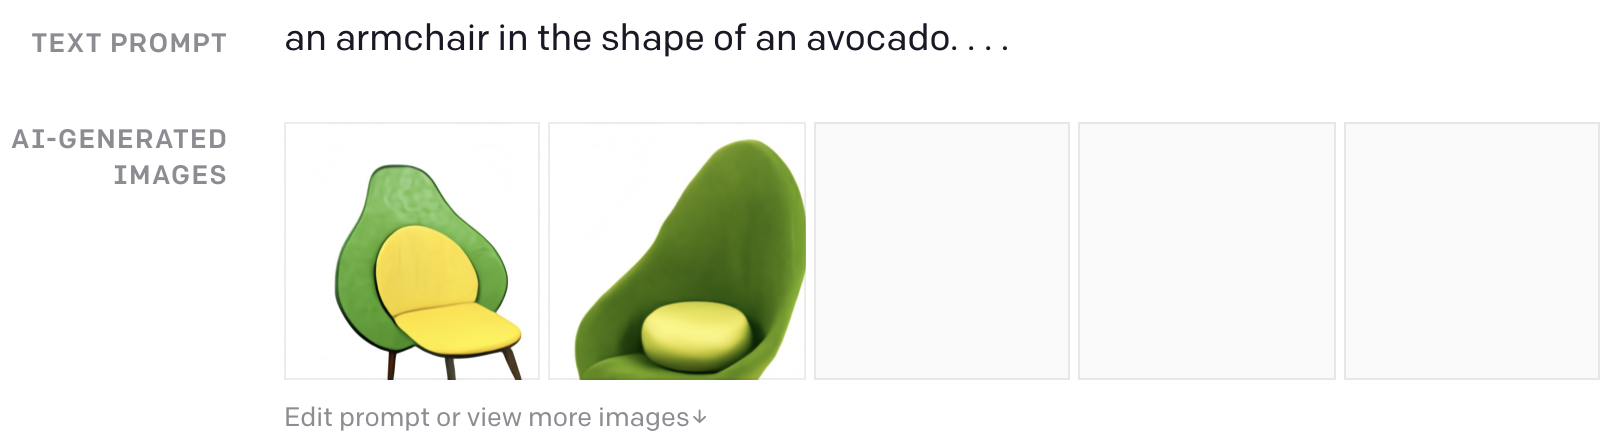
\includegraphics[width=\linewidth]{figs/dalle1}
	\end{figure}
	\vspace{-0.5cm}
	\begin{figure}
		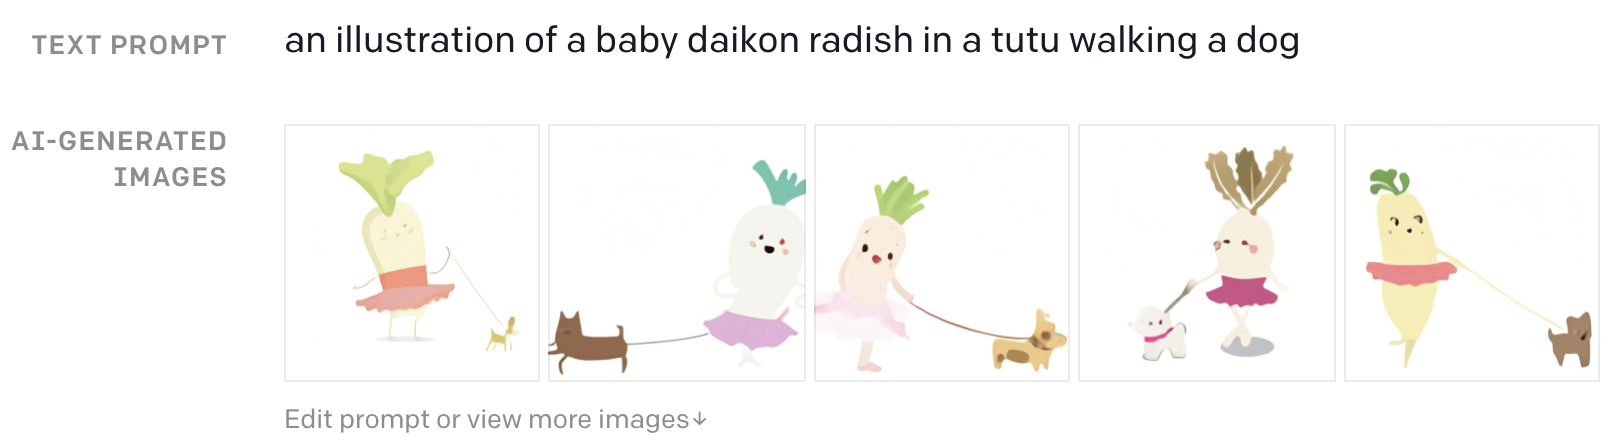
\includegraphics[width=\linewidth]{figs/dalle2}
	\end{figure}
	\myfootnote{\href{https://openai.com/blog/dall-e/}{image credit: https://openai.com/blog/dall-e/} \\
		\href{https://arxiv.org/abs/2102.1209}{Ramesh A. et al. Zero-shot text-to-image generation, 2021}}
\end{frame}
%=======
\begin{frame}{Applications: Image generation}
	\begin{figure}
		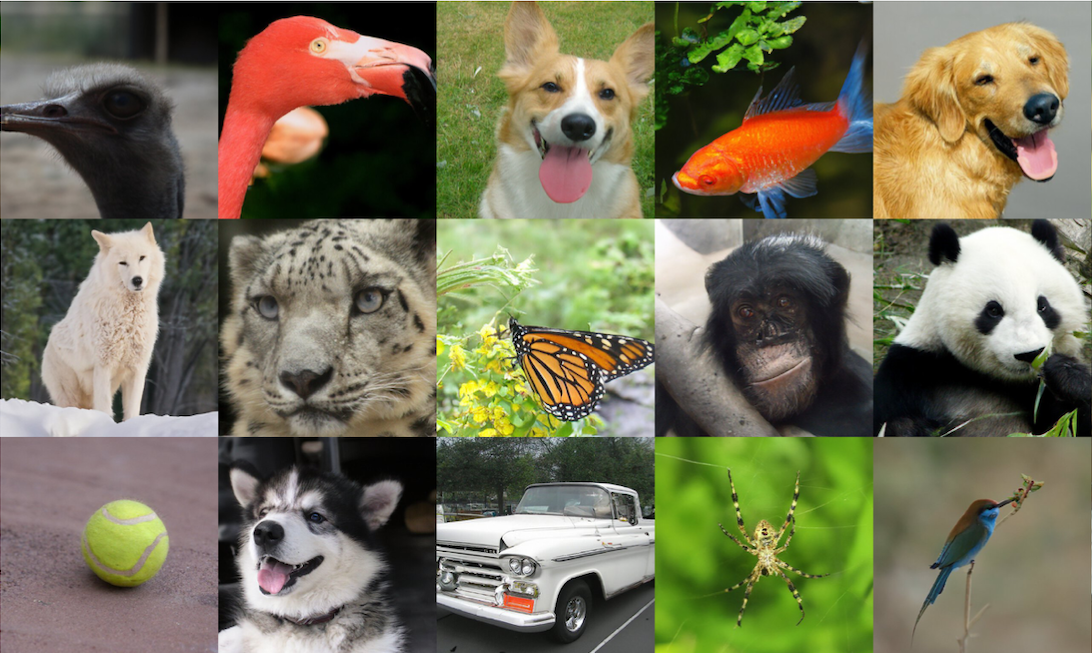
\includegraphics[width=\linewidth]{figs/diffusion_models}
	\end{figure}
	\myfootnotewithlink{https://arxiv.org/abs/2105.05233}{Dhariwal P., Nichol A. Diffusion Models Beat GANs on Image Synthesis, 2021}
\end{frame}
%=======
\begin{frame}{Problem Statement}
We are given i.i.d. samples $\{\bx_i\}_{i=1}^n \in X$ (e.g. $X = \bbR^m$) from unknown distribution $\pi(\bx)$.

\begin{block}{Goal}
	We would like to learn a distribution $\pi(\bx)$ for 
	\begin{itemize}
	    \item evaluating $\pi(\bx)$ for new samples (how likely to get object $\bx$?);
	    \item sampling from $\pi(\bx)$ (to get new objects $\bx \sim \pi(\bx)$).
	\end{itemize}
\end{block}
\begin{block}{Challenge}
	 Data is complex and high-dimensional. E.g. the dataset of images lies in the space $X \subset \bbR^{\text{width} \times \text{height} \times \text{channels}}$.
\end{block}
\end{frame}
%=======
\begin{frame}{Histogram as a generative model}
	
	\begin{minipage}[t]{0.6\columnwidth}
	    Let $x \sim \text{Categorical}(\bpi)$. The histogram is totally defined by
		\[
		    \pi_k = \pi(x = k) = \frac{\sum_{i=1}^k [x_i = k]}{n}.
		\]
		\textbf{Problem:} curse of dimensionality (number of bins grows exponentially). \\
		\end{minipage}%
		\begin{minipage}[t]{0.4\columnwidth}
	    \begin{figure}[h]
	        \centering
	        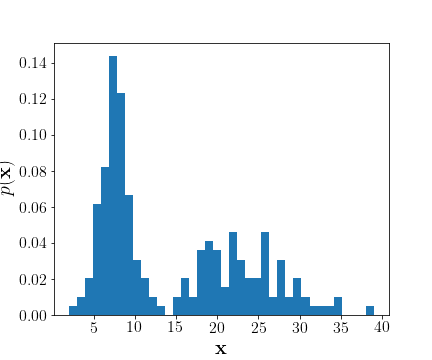
\includegraphics[width=\linewidth]{figs/histogram.png}
	    \end{figure}
	\end{minipage}
	\textbf{MNIST example}: 28x28 gray-scaled images, each image is $\bx = (x_1, \dots, x_{784})$, where $x_i = \{0, 1\}$. 
	\[
	    \pi(\bx) = \pi(x_1) \cdot \pi(x_2 | x_1) \cdot \dots \cdot \pi(x_m | x_{m-1}, \dots, x_1).
	\]
	Hence, the histogram will have $2^{28 \times 28} - 1$ parameters to specify $\pi(\bx)$. \\
	\textbf{Question:} How many parameters do we need in these cases?
	\begin{align*}
	    \pi(\bx) &= \pi(x_1) \cdot \pi(x_2)\cdot \dots \cdot \pi(x_m); \\
	    \pi(\bx) &= \pi(x_1) \cdot \pi(x_2 | x_1) \cdot \dots \cdot \pi(x_m | x_{m-1}).
	\end{align*}
\end{frame}
%=======
\begin{frame}{Tricks}
	\begin{block}{Monte-Carlo estimation}
		\vspace{-0.5cm}
		\[
			\bbE_{p(\bx)} f(\bx) = \int p(\bx) f(\bx) d \bx \approx \frac{1}{n} \sum_{i=1}^n f(\bx_i), \quad 
			\text{where } \bx_i \sim p(\bx).
		\]
		Integral of expected value could be estimated using only samples from the distribution.
	\end{block}
	\begin{block}{Law of the unconscious statistician (LOTUS)}
		Let $X$ be a random variable and let $Y=g(X)$. Then
		\[
			\bbE_{p_Y} Y = \bbE_{p_X} g(X) = \int g(\bx) p(\bx) d \bx.
		\]
		The name LOTUS came from a purported tendency to use the identity without realizing that it must be treated as the result of a rigorously proved theorem, not merely a definition.
	\end{block}
\end{frame}
%=======
\begin{frame}{Divergences}
	Fix probabilistic model $p(\bx | \btheta)$~-- the set of parameterized distributions. \\
	Instead of searching true $\pi(\bx)$ over all probability distributions, learn function approximation $p(\bx | \btheta) \approx \pi(\bx)$.
	\begin{block}{What is a divergence?}
		Let $\cS$ be the set of all possible probability distributions. Then $D: \cS \times \cS \rightarrow \bbR$ is a divergence if 
		\begin{itemize}
			\item $D(\pi || p) \geq 0$ for all $\pi, p \in \cS$;
			\item $D(\pi || p) = 0$ if and only if $\pi \equiv p$.
		\end{itemize}
	\end{block}
	\begin{block}{General divergence minimization task}
		\vspace{-0.3cm}
		\[
		\min_{\btheta} D(\pi || p),
		\]
		where $\pi(\bx)$ is a true data distribution, $p(\bx | \btheta)$ is a model distribution.
	\end{block}
\end{frame}
%=======
\begin{frame}{f-divergence family}
	
	\begin{block}{f-divergence}
		\vspace{-0.3cm}
		\[
		D_f(\pi || p) = \bbE_{p(\bx)}  f\left( \frac{\pi(\bx)}{p(\bx)} \right)  = \int p(\bx) f\left( \frac{\pi(\bx)}{p(\bx)} \right) d \bx.
		\]
		Here $f: \bbR_+ \rightarrow \bbR$ is a convex, lower semicontinuous function satisfying $f(1) = 0$.
	\end{block}
	\begin{figure}
		\centering
		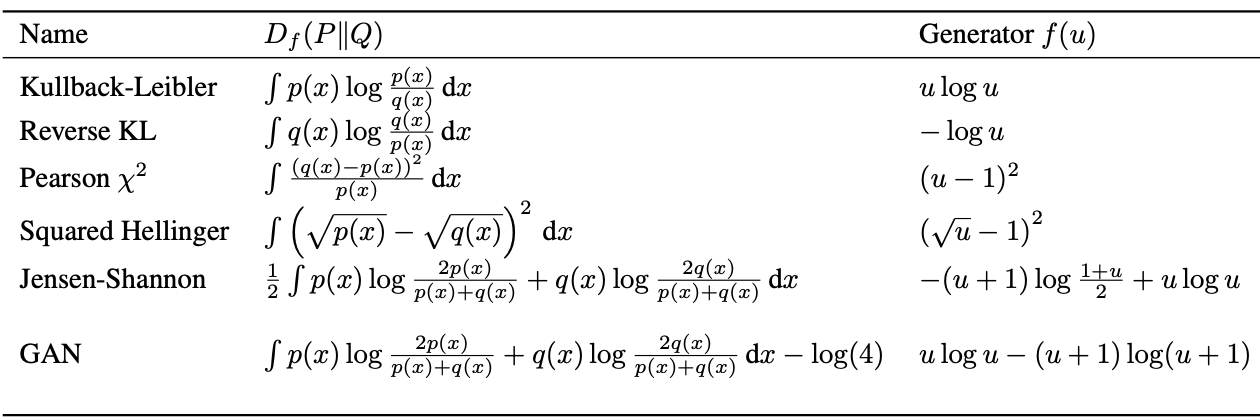
\includegraphics[width=\linewidth]{figs/f_divs}
	\end{figure}
	\myfootnotewithlink{https://arxiv.org/abs/1606.00709}{Nowozin S., Cseke B., Tomioka R. f-GAN: Training Generative Neural Samplers using Variational Divergence Minimization, 2016}
\end{frame}
%=======
\begin{frame}{Forward KL vs Reverse KL}
	\begin{block}{Forward KL}
		\vspace{-0.2cm}
		\[
		KL(\pi || p) = \int \pi (\bx) \log \frac{\pi(\bx)}{p(\bx | \btheta)} d \bx \rightarrow \min_{\btheta}
		\]
	\end{block}
	\begin{block}{Reverse KL}
		\vspace{-0.2cm}
		\[
		KL(p || \pi) = \int p (\bx| \btheta) \log \frac{p(\bx| \btheta)}{\pi(\bx)} d \bx \rightarrow \min_{\btheta}
		\]
	\end{block}
	What is the difference between these two formulations?
	
	\begin{block}{Maximum likelihood estimation (MLE)}
		\vspace{-0.5cm}
		\[
		\btheta^* = \argmax_{\btheta} p(\bX | \btheta) = \argmax_{\btheta} \prod_{i=1}^n p(\bx_i | \btheta) = \argmax_{\btheta} \sum_{i=1}^n \log p(\bx_i | \btheta).
		\]
		\vspace{-0.1cm}
	\end{block}
\end{frame}
%=======
\begin{frame}{Forward KL vs Reverse KL}
	\begin{block}{Forward KL}
		\vspace{-0.5cm}
		\begin{align*}
			KL(\pi || p) &= \int \pi (\bx) \log \frac{\pi(\bx)}{p(\bx | \btheta)} d \bx \\
			&= \int \pi (\bx) \log \pi(\bx) d \bx - \int \pi (\bx) \log p(\bx | \btheta) d \bx \\
			&= - \bbE_{\pi(\bx)} \log p(\bx | \btheta) + \text{const} \\
			& \approx - \frac{1}{n} \sum_{i=1}^n \log p(\bx_i | \btheta) + \text{const} \rightarrow \min_{\btheta}.
		\end{align*}
		\vspace{-0.5cm}
	\end{block}
	Maximum likelihood estimation is equivalent to minimization of the Monte-Carlo estimate of forward KL.
	\begin{block}{Reverse KL}
		\vspace{-0.5cm}
		\begin{align*}
			KL(p || \pi) &= \int p(\bx | \btheta) \log \frac{p(\bx | \btheta)}{\pi(\bx)} d \bx \\
			&= \bbE_{p(\bx | \btheta)} \left[\log p(\bx | \btheta) - \log \pi(\bx)\right] \rightarrow \min_{\btheta}
		\end{align*}
		\vspace{-0.7cm}
	\end{block}
\end{frame}
%=======
\begin{frame}{Autoregressive model}
    \begin{block}{MLE problem}
	    \vspace{-0.7cm}
	    \[
	        \btheta^* = \argmax_{\btheta} p(\bX | \btheta) = \argmax_{\btheta} \prod_{i=1}^n p(\bx_i | \btheta) = \argmax_{\btheta} \sum_{i=1}^n \log p(\bx_i | \btheta).
	    \]
	    \vspace{-0.5cm}
    \end{block}
    \begin{itemize}
        \item We would like to solve the problem using gradient-based optimization.
        \item We have to efficiently compute $\log p(\bx | \btheta)$ and $\frac{\partial \log p(\bx | \btheta)}{\partial \btheta}$.
    \end{itemize}
    \begin{block}{Likelihood as product of conditionals}
    Let $\bx = (x_1, \dots, x_m)$, $\bx_{1:i} = (x_1, \dots, x_i)$. Then 
    \[
        p(\bx | \btheta) = \prod_{i=1}^m p(x_i | \bx_{1:i - 1}, \btheta); \quad 
        \log p(\bx | \btheta) = \sum_{i=1}^m \log p(x_i | \bx_{1:i - 1}, \btheta).
    \]
    \end{block}
	\textbf{Example:} $p(x_1, x_2, x_3) = p(x_2) \cdot p(x_1 | x_2) \cdot p(x_3 | x_1, x_2)$.
\end{frame}
%=======
\begin{frame}{Autoregressive models}
    \[
    \log p(\bx| \btheta) = \sum_{i=1}^m \log p(x_i | \bx_{1:i - 1}, \btheta)
    \]
    \begin{itemize}
	    \item Sampling is sequential:
	    \begin{itemize}
    		\item sample $\hat{x}_1 \sim p(x_1 | \btheta)$;
    		\item sample $\hat{x}_2 \sim p(x_2 | \hat{x}_1, \btheta)$;
    		\item \dots
    		\item sample $\hat{x}_m \sim p(x_n | \hat{\bx}_{1:m-1}, \btheta)$;
    		\item new generated object is $\hat{\bx} = (\hat{x}_1, \hat{x}_2, \dots, \hat{x}_m)$.
    	\end{itemize}
        \item Each conditional $p(x_i | \bx_{1:i - 1}, \btheta)$ could be modelled by neural network.
        \item Modelling all conditional distributions separately is infeasible and we would obtain separate models. To extend to high dimensions we could share parameters $\btheta$ across conditionals.

    \end{itemize}
\end{frame}
%=======
\begin{frame}{Autoregressive models}
		For large $i$ the conditional distribution $p(x_i | \bx_{1:i - 1}, \btheta)$ could be infeasible. Moreover, the history $\bx_{1:i-1}$ has non-fixed length.
		\begin{block}{Markov assumption}
			\vspace{-0.5cm}
			\[
				p(x_i | \bx_{1:i - 1}, \btheta) = p(x_i | \bx_{i - d:i - 1}, \btheta), \quad d \text{ is a fixed model parameter}.
			\]
		\end{block}
		\vspace{-0.5cm}
		\begin{block}{Example}
			\begin{minipage}[t]{0.39\columnwidth}
				{\small
				\begin{itemize}
					\item $d = 2$;
					\item $x_i \in \{0, 255\}$;
					\item $\bh_i = \text{MLP}_{\btheta}(x_{i - 1}, x_{i - 2})$;
					\item $\bpi_i = \text{softmax}(\bh_i)$;
					\item $p(x_i | x_{i - 1}, x_{i - 2}, \btheta) = \text{Categorical}(\bpi_i)$.
				\end{itemize}
				}
			\end{minipage}%
			\begin{minipage}[t]{0.61\columnwidth}
	   \begin{figure}
	       \centering
	       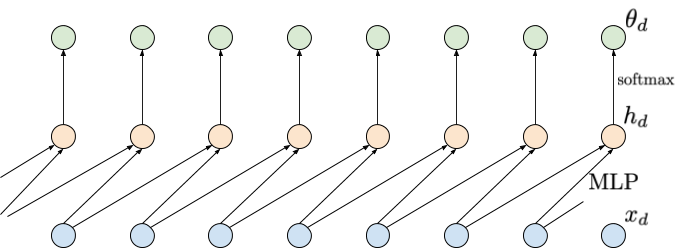
\includegraphics[width=1.0\linewidth]{figs/sequential_MLP}
	   \end{figure}
			\end{minipage}
		\end{block}
	 \myfootnotewithlink{https://jmtomczak.github.io/blog/2/2\_ARM.html}{image credit: https://jmtomczak.github.io/blog/2/2\_ARM.html}
\end{frame}
%=======
\begin{frame}{Autoregressive models}
	\begin{itemize}
		\item Previous model has \textbf{limited} memory $d$. It is insufficient for many modalities (e.g. for images and text). 
		\item Recurrent NN fixes this problem and potentially could learn long-range dependencies:
		\[
			p(x_i | \bx_{1:i - 1}, \btheta) = p(x_i | \bh_i, \btheta), \quad \bh_i = \text{RNN}(\bx_{i - 1}, \bh_{i - 1})
		\]
		 \begin{figure}
	    \centering
	    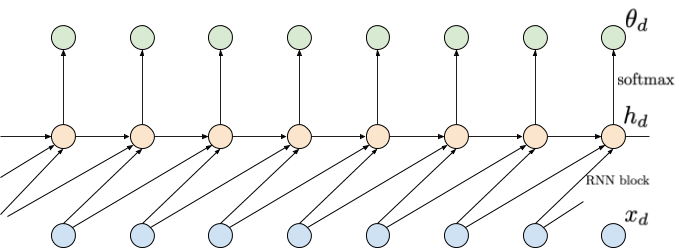
\includegraphics[width=0.7\linewidth]{figs/sequential_RNN}
		 \end{figure}
		\item Sequential computation of all conditionals $p(x_i | \bx_{1:i-1}, \btheta)$, hence, the training is slow.
		\item RNN suffers from vanishing and exploding gradients.
	\end{itemize}
	 \myfootnotewithlink{https://jmtomczak.github.io/blog/2/2\_ARM.html}{image credit: https://jmtomczak.github.io/blog/2/2\_ARM.html}
\end{frame}
%=======
\begin{frame}{Char RNN}
	Model tries to predict the next token (single letter) from previous context.
	\begin{minipage}[t]{0.55\columnwidth}
		\begin{figure}
			\centering
			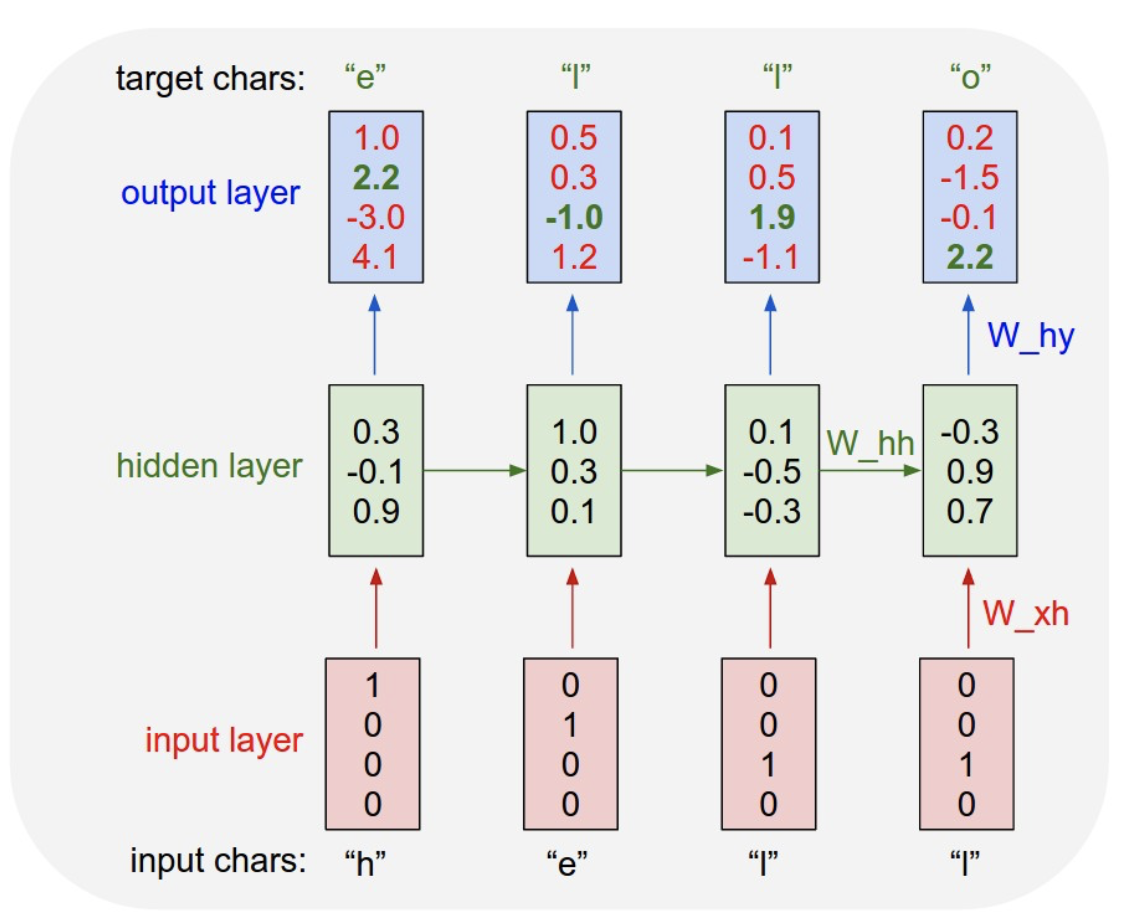
\includegraphics[width=1.0\linewidth]{figs/char_rnn.png}
		\end{figure}
	\end{minipage}%
	\begin{minipage}[t]{0.44\columnwidth}
		\begin{figure}
			\centering
			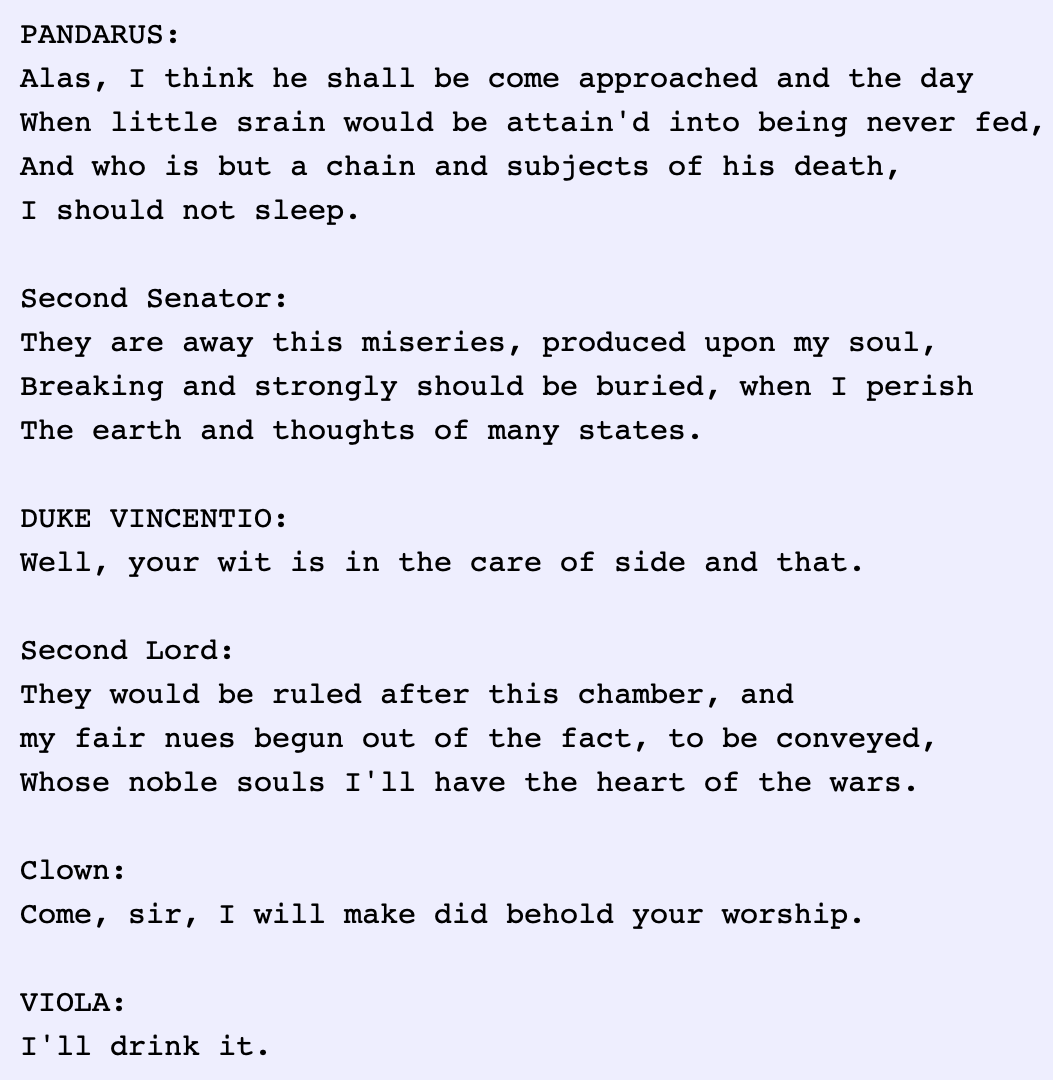
\includegraphics[width=1.0\linewidth]{figs/char_rnn_output.png}
		\end{figure}
	\end{minipage}
\myfootnotewithlink{http://karpathy.github.io/2015/05/21/rnn-effectiveness/}{image credit: http://karpathy.github.io/2015/05/21/rnn-effectiveness}
\end{frame}
%=======
\begin{frame}{Autoregressive models}
		\begin{itemize}
			\item Convolutions could be used for autoregressive models, but they have to be \textbf{causal}. \\
			\item Try to find and understand the difference between Conv A/B.
		    \begin{figure}
		        \centering
		        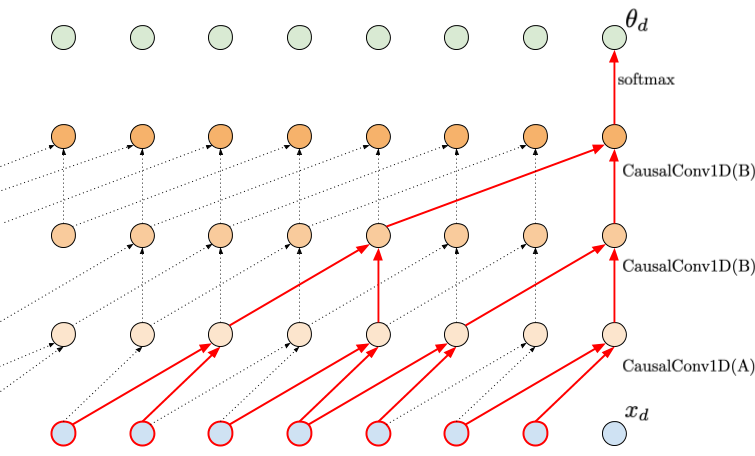
\includegraphics[width=0.7\linewidth]{figs/sequential_CNN}
		    \end{figure}
		    \item Could learn long-range dependecies.
		    \item Do not suffer from gradient issues.
		    \item Easy to estimate probability for given input, but hard generation of new samples (the sequential process).
	   	\end{itemize}
	    \myfootnotewithlink{https://jmtomczak.github.io/blog/2/2\_ARM.html}{image credit: https://jmtomczak.github.io/blog/2/2\_ARM.html}
\end{frame}
%=======
\begin{frame}{MADE}
	\begin{itemize}
		\item Vanila autoencoder is not a generative model. Why?
		\item Let mask the weight matrices to make the model generative: $\bW_M = \bW \cdot \bM$.
		\begin{figure}
		    \centering
		    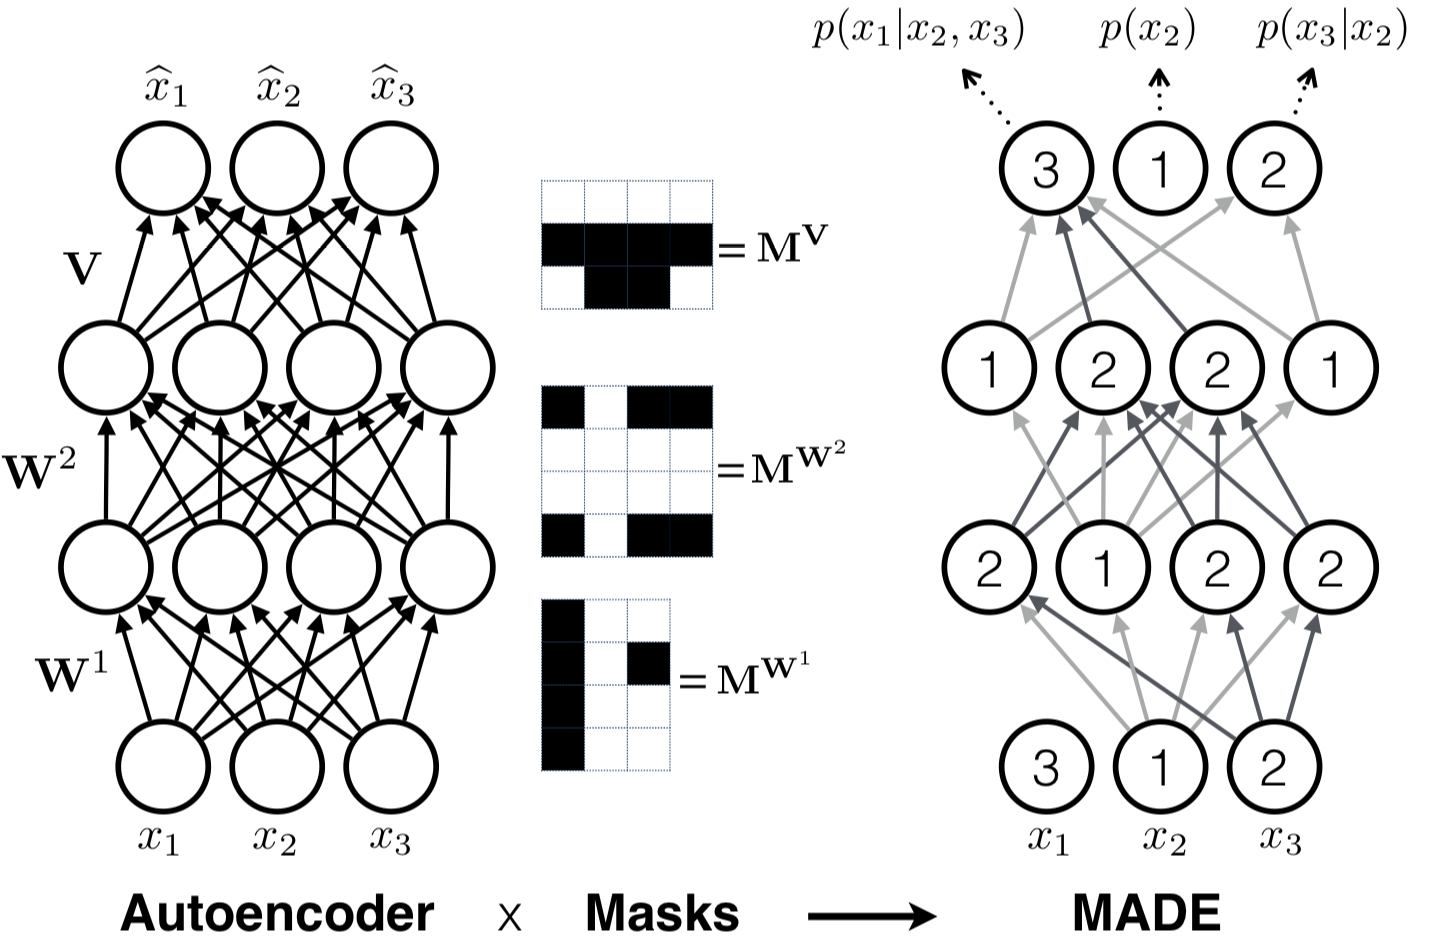
\includegraphics[width=0.7\linewidth]{figs/made}
		\end{figure}
		\item The question is how to create matrices $\bM$ which produce the autoregressive property?
	\end{itemize}
	\myfootnotewithlink{https://arxiv.org/abs/1502.03509}{Germain M. et al. Made: Masked autoencoder for distribution estimation, 2015}
\end{frame}
%=======
\begin{frame}{MADE}
		\begin{minipage}[t]{0.65\columnwidth}
		    \vspace{-0.5cm}
			\begin{block}{Masks generation}
				\begin{itemize}
					\item Define the ordering of input elements from 1 to $m$.
					\item Assign the random number $k$ from 1 to $m - 1$ to each hidden unit. The number gives the
					maximum number of input units to which the unit can be connected.
					\item Connect each hidden unit with number $k$ with the previous layer units which has the number is \textbf{less or equal} than~$k$.
					\item Connect each output unit with number $k$ with the previous layer units which has the number is \textbf{less} than $k$.
				\end{itemize}
			\end{block}
		\end{minipage}%
		\begin{minipage}[t]{0.33\columnwidth}
			\vspace{2cm}
			\begin{figure}
				\centering
				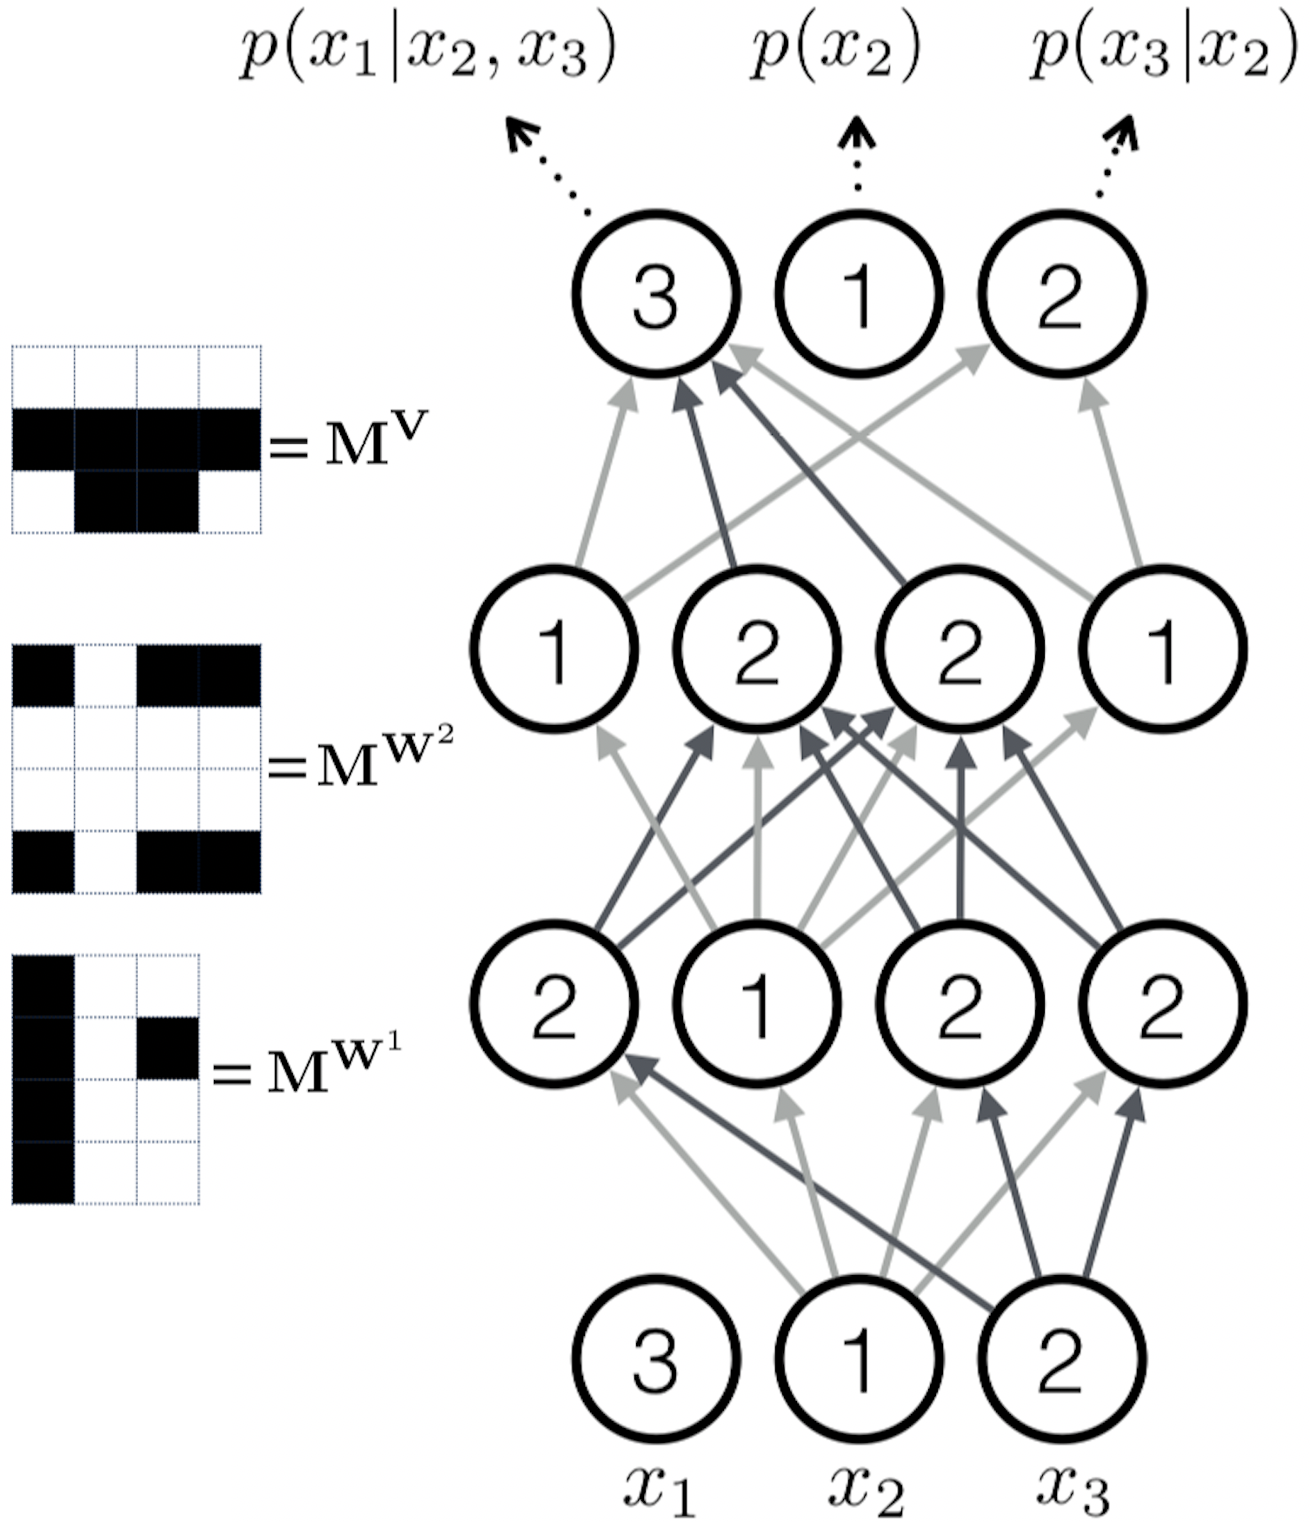
\includegraphics[width=1.0\linewidth]{figs/made2}
			\end{figure}
		\end{minipage}
	\myfootnotewithlink{https://arxiv.org/abs/1502.03509}{Germain M. et al. Made: Masked autoencoder for distribution estimation, 2015}
\end{frame}
%=======
\begin{frame}{MADE}
	\begin{block}{Possible variations}
		\begin{itemize}
			\item Order agnostic training (missing values in partially observed input vectors can be imputed efficiently);
			\item Connectivity-agnostic training (cheap ensembling).
		\end{itemize}
	\end{block}
	\vspace{-0.3cm}
	\begin{minipage}[t]{0.59\columnwidth}
		\begin{figure}
			  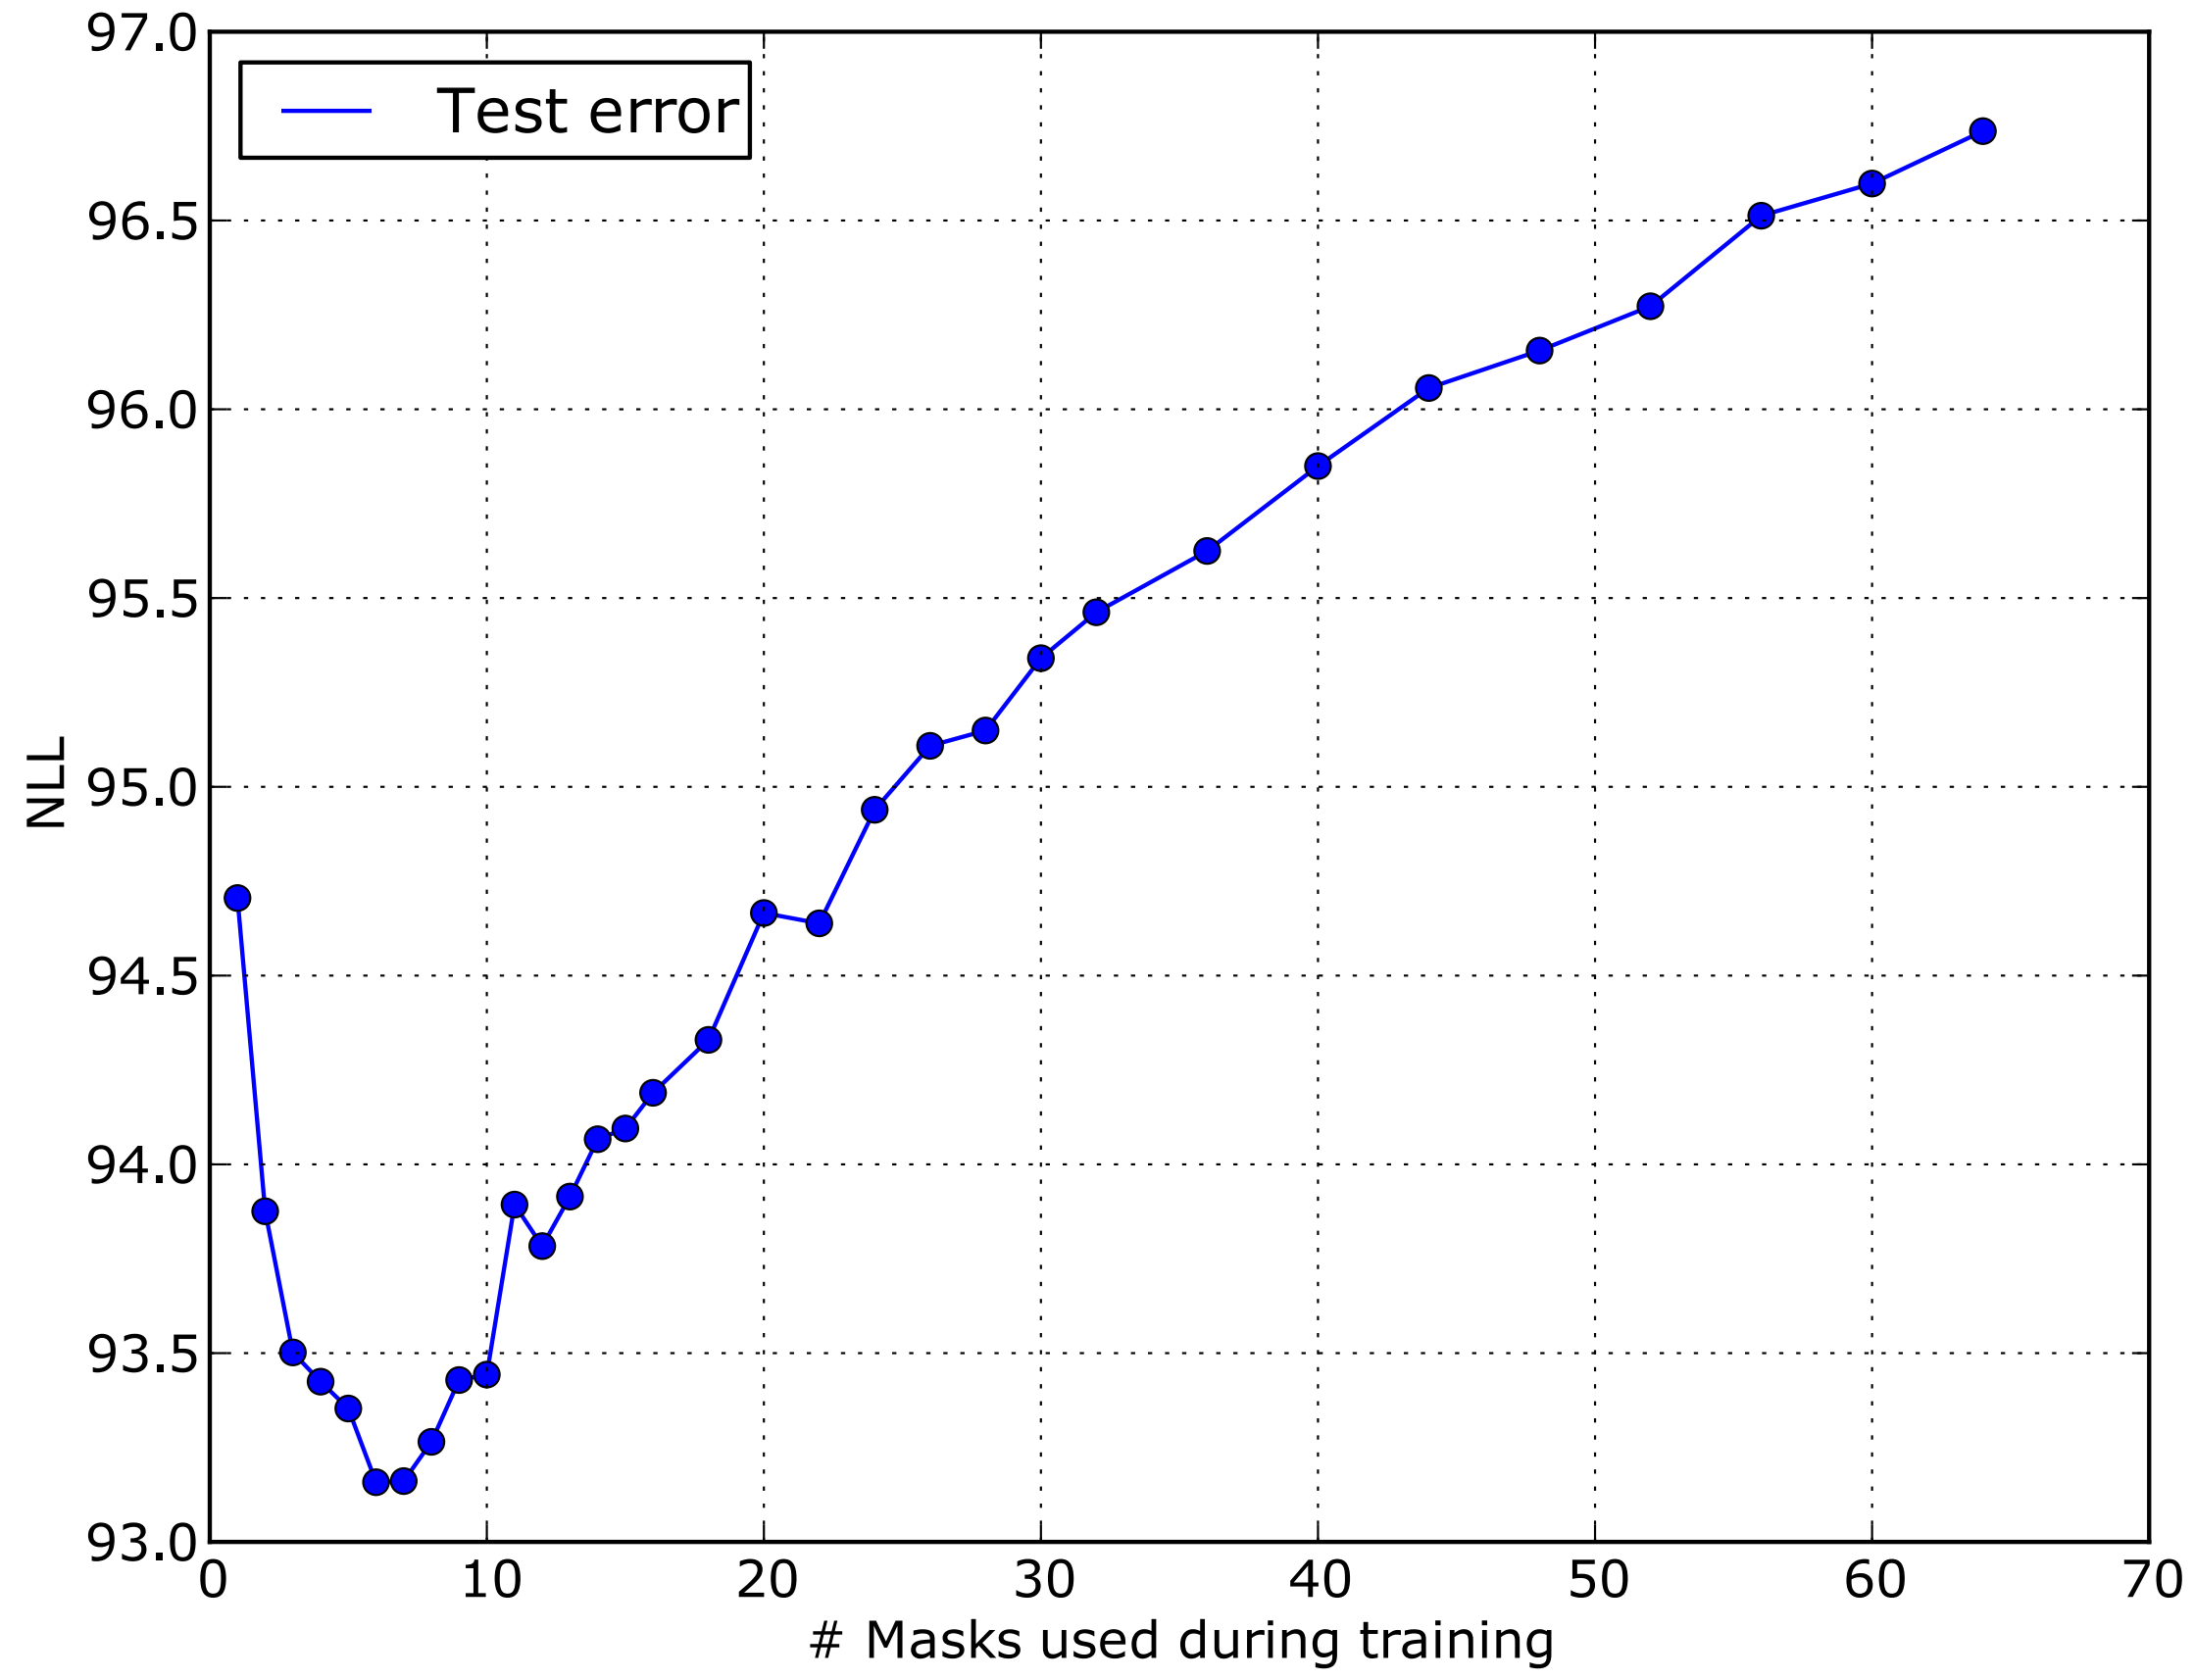
\includegraphics[width=\linewidth]{figs/made_nmasks}
		\end{figure}
	\end{minipage}%
	\begin{minipage}[t]{0.41\columnwidth}
		\begin{figure}
	  		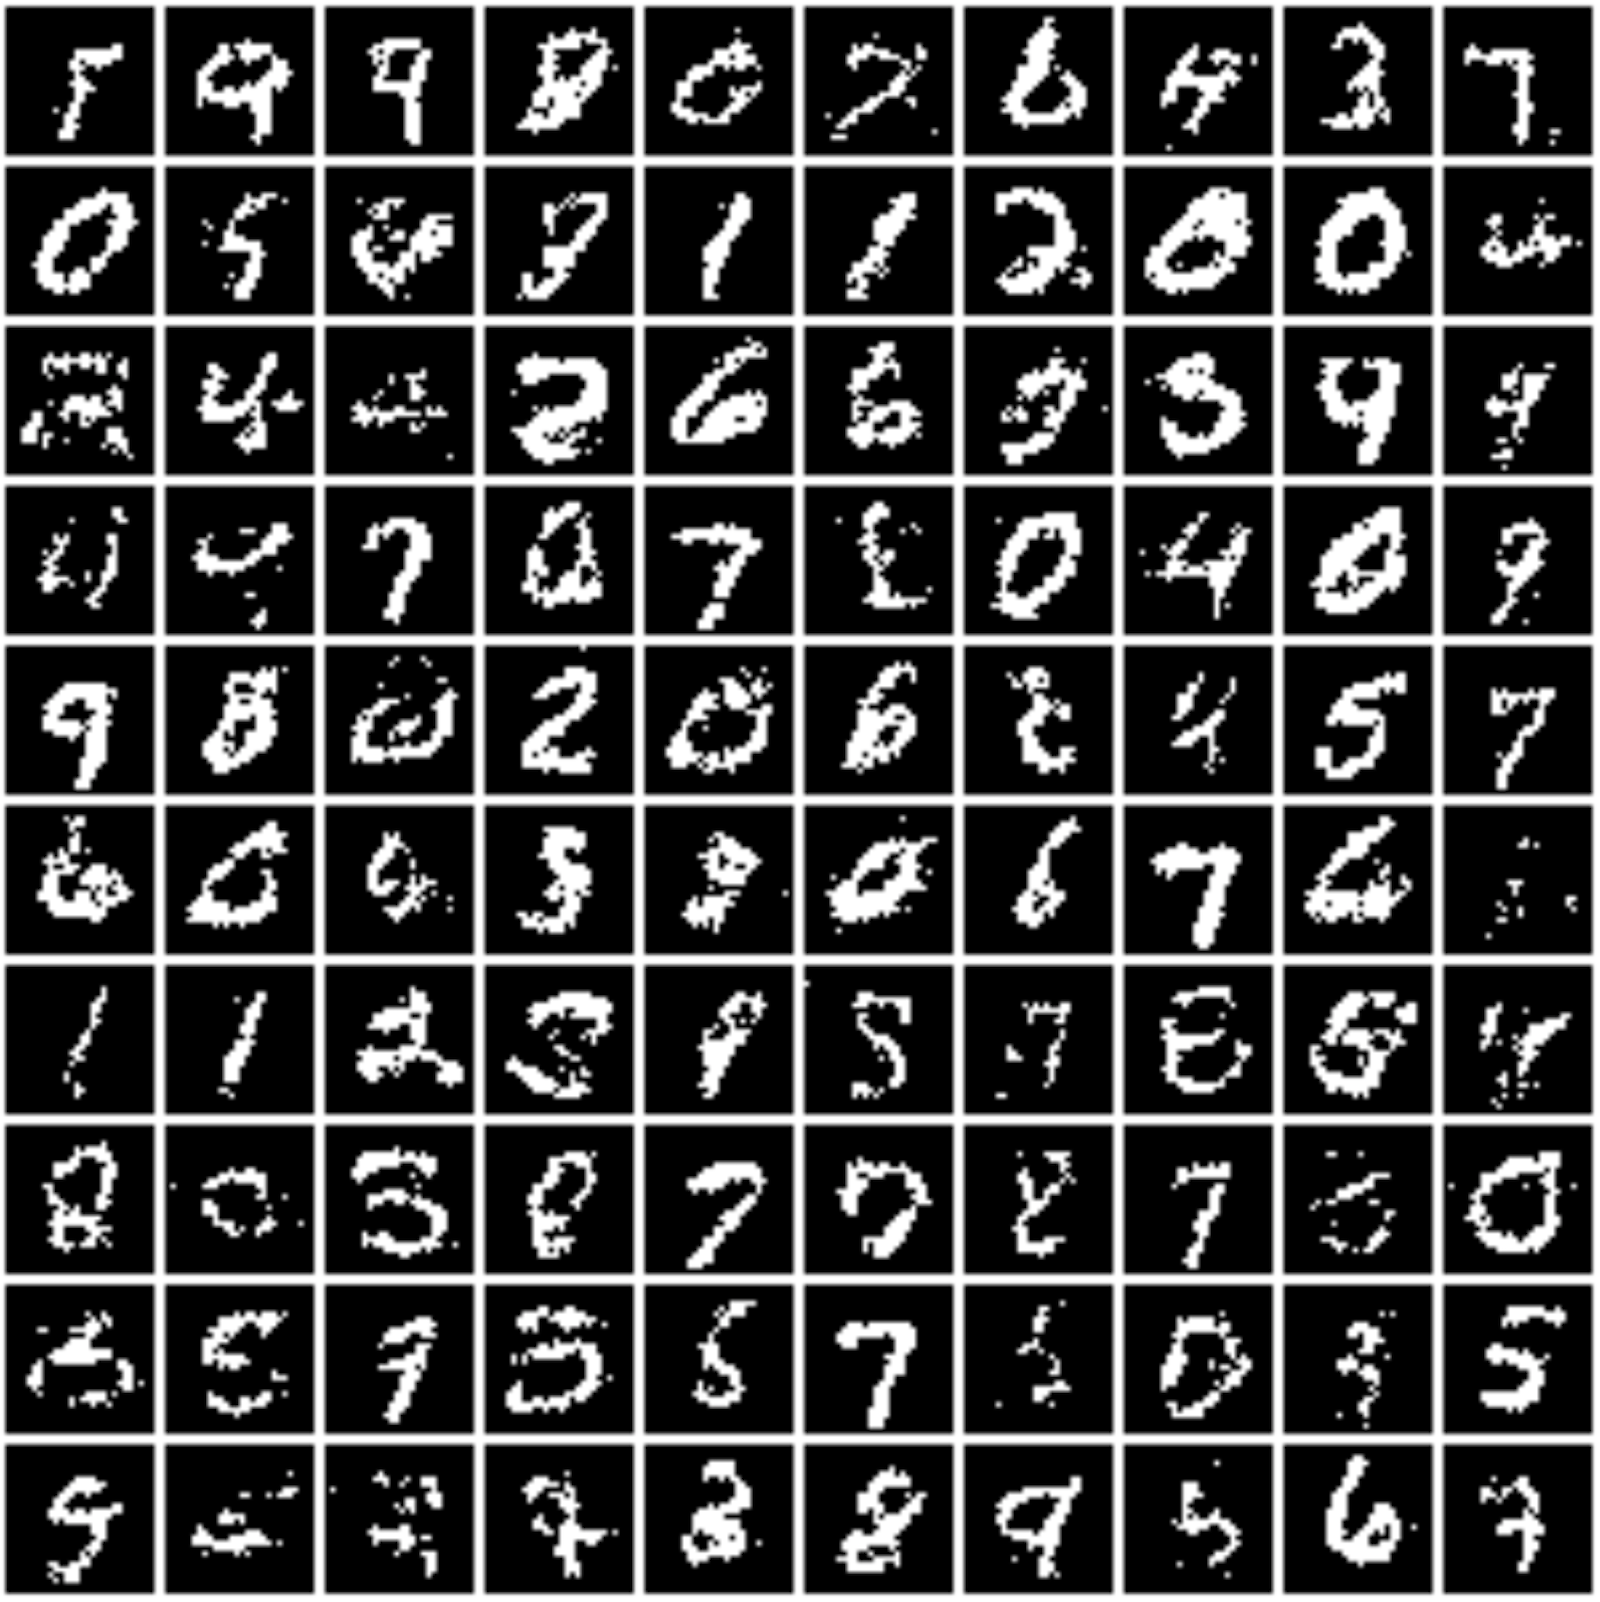
\includegraphics[width=\linewidth]{figs/made_results}
		\end{figure}
	\end{minipage}
	\myfootnotewithlink{https://arxiv.org/abs/1502.03509}{Germain M. et al. Made: Masked autoencoder for distribution estimation, 2015}
\end{frame}
%=======
\begin{frame}{Summary}
    \begin{itemize}
    	\item We are trying to approximate the distribution of samples for density estimation and generation of new samples.
    	\item To fit model distribution to the real data distribution one could use divergence minimization framework.
    	\item Minimization of forward KL is equivalent to the MLE problem.
    	\item Autoregressive models decompose the distribution to the sequence of conditionals.
        \item Sampling from autoregressive models is trivial, but sequential
        \begin{itemize}
            \item sample $x_1 \sim p(x_1)$;
            \item sample $x_2 \sim p(x_2 | x_1)$;
            \item \dots.
        \end{itemize}
        \item Density estimation:
        \vspace{-0.2cm}
        \[
            p(\bx) = \prod_{i=1}^m p(x_i | \bx_{1:i - 1}).
        \]
        \vspace{-0.2cm}
        \item Autoregressive models work on both continuous and discrete data.
    \end{itemize}
\end{frame}

\end{document} 